\section{Цель работы}
Исследовать схемы базовых логических элементов (НЕ, И, ИЛИ, НЕ-И, НЕ-ИЛИ), реализованных в 6 типах логических семейств:
\begin{itemize}
    \item диодно-резисторная логика (DRL),
    \item резисторно-транзисторная логика (RTL),
    \item диодно-транзисторная логика (DTL),
    \item транзисторно-транзисторная логика (TTL),
    \item логика на МОП-транзисторах одного типа (MOS),
    \item комплементарная МОП-логика (CMOS).
\end{itemize}

\section{Исходные данные}
\begin{tabular}{|c|c|c|c|c|c|c|}
\hline
№ & Логика 1 & Элементы & Логика 2 & Элементы & Логика 3 & Элементы \\
\hline
3 & TTL & НЕ, НЕ-И & DTL & ИЛИ, И & MOS & НЕ, ИЛИ \\
\hline
\end{tabular}

\section{Сборка схем логических элементов}
Ниже представлены схемы исследуемых элементов:

\begin{figure}[H]
    \centering
    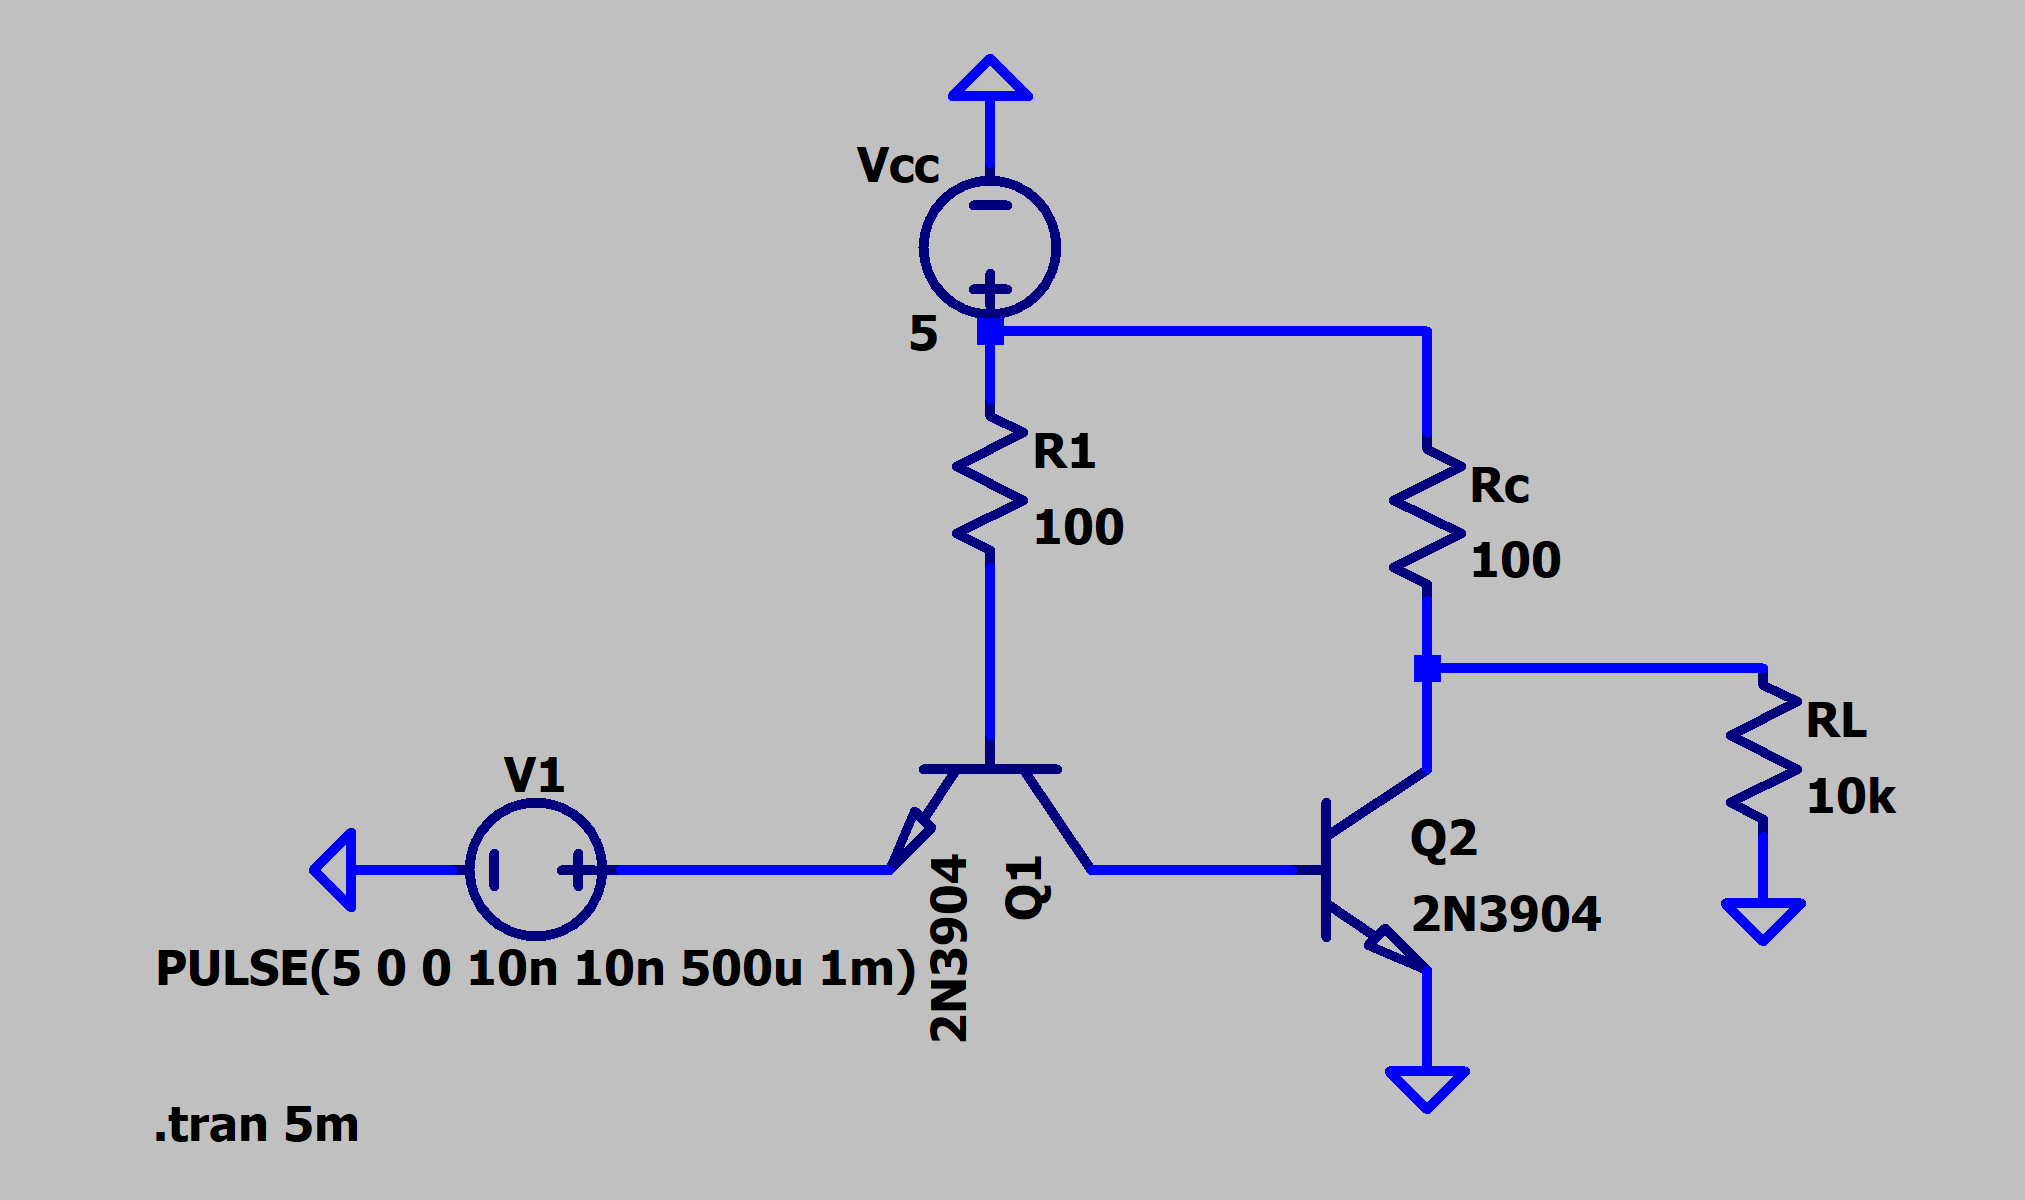
\includegraphics[width=0.5\textwidth]{images/TTL_NOT.png}
    \caption{TTL NOT}
    \label{TTL_NOT}
\end{figure}
\begin{figure}[H]
    \centering
    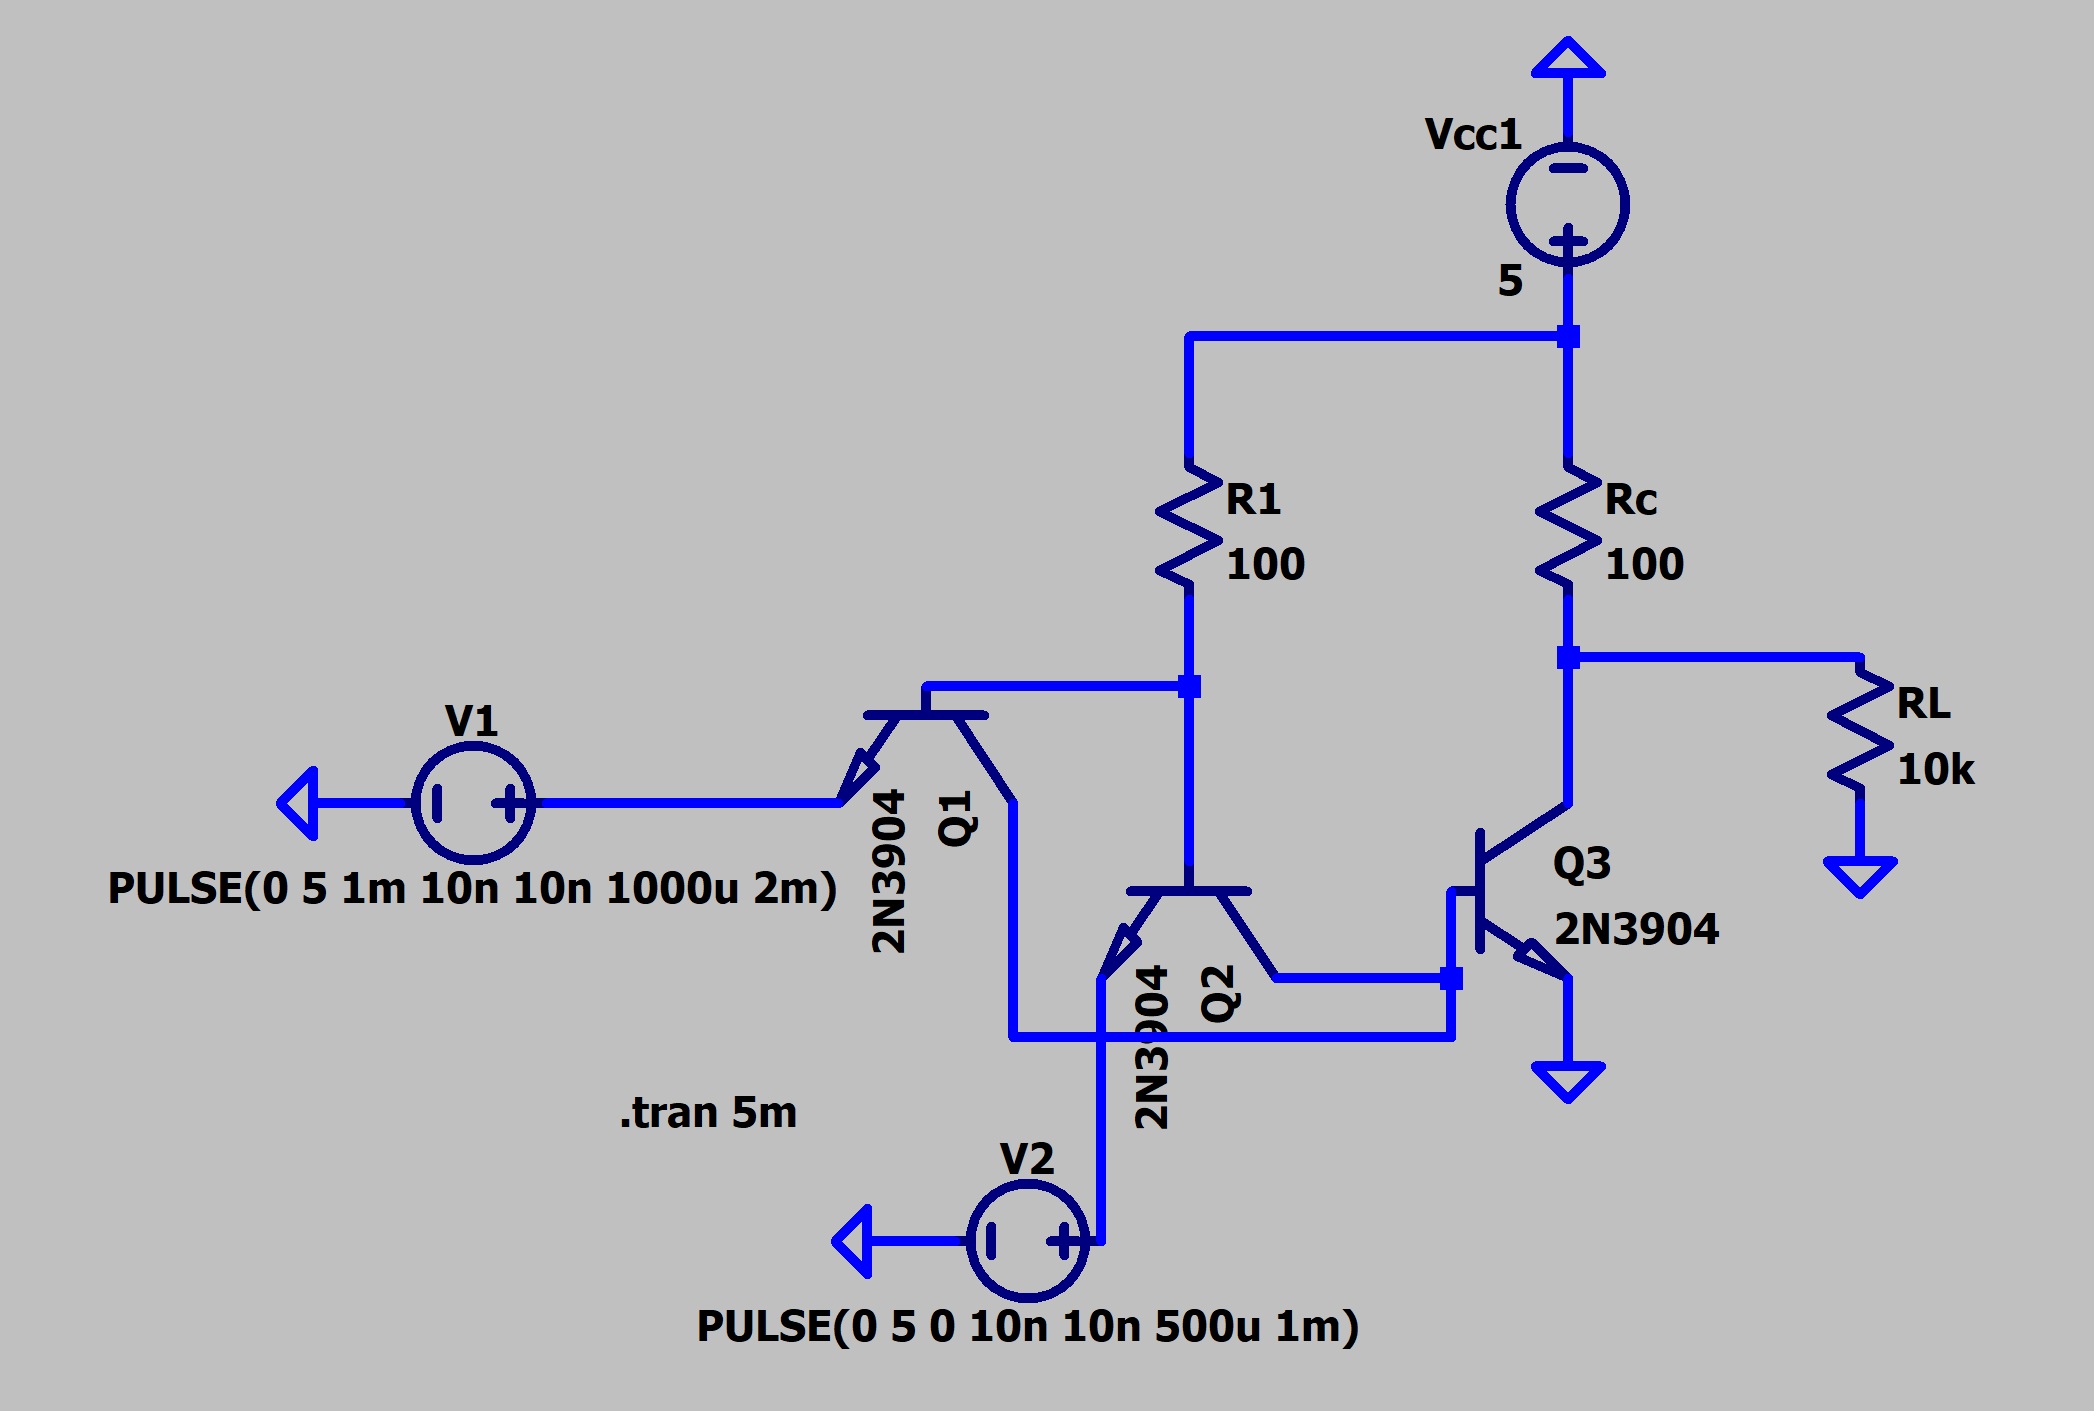
\includegraphics[width=0.5\textwidth]{images/TTL_NAND.png}
    \caption{TTL NAND}
    \label{TTL_NAND}
\end{figure}
\begin{figure}[H]
    \centering
    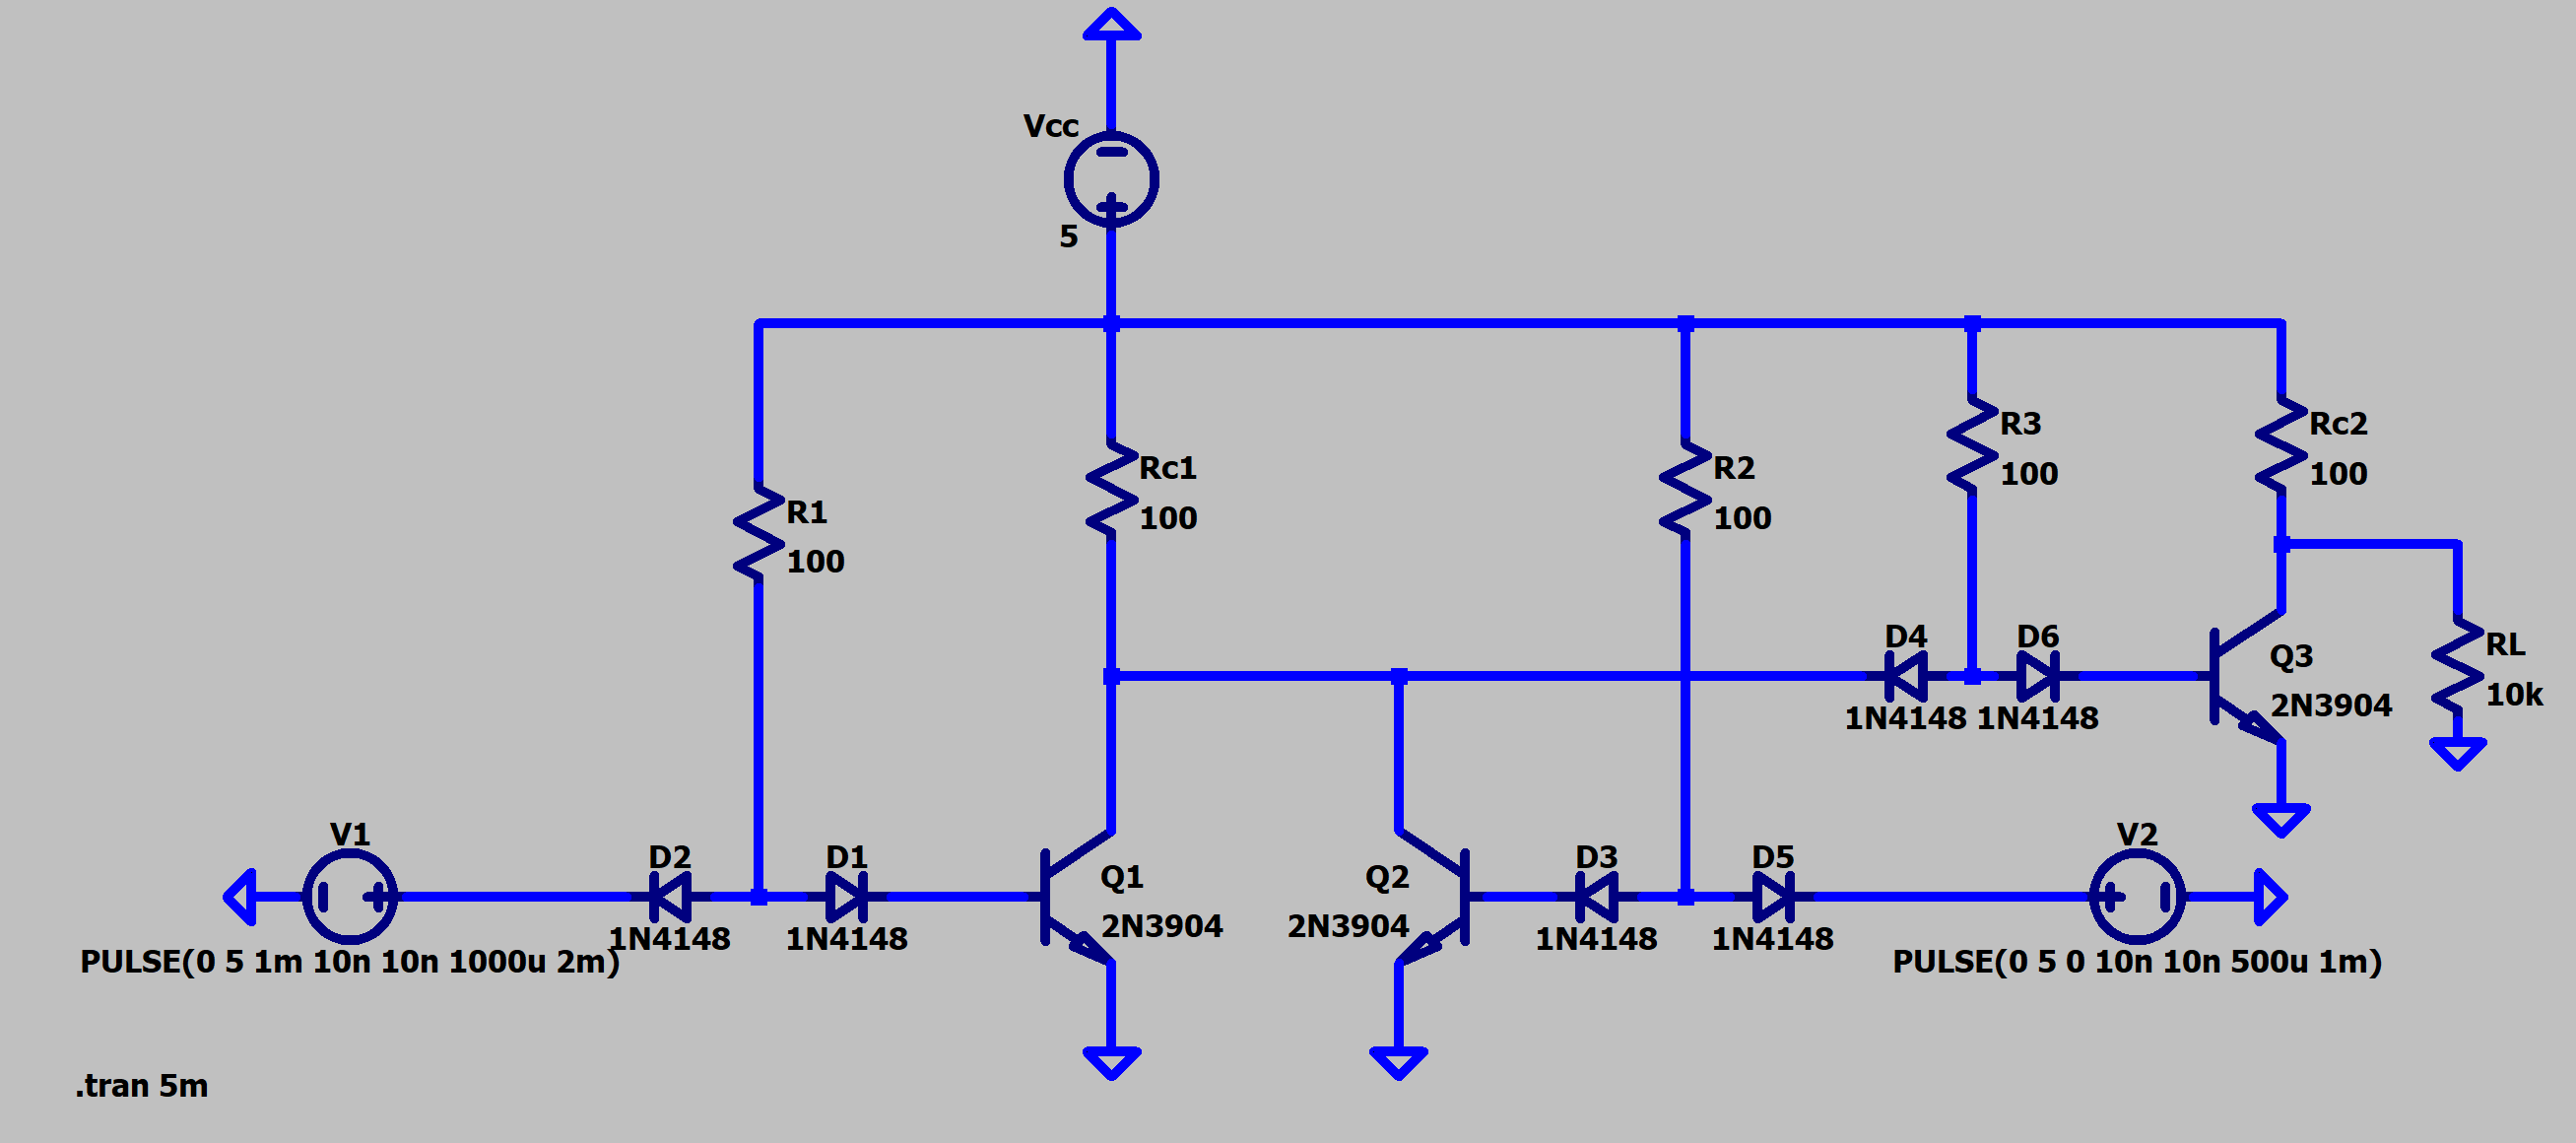
\includegraphics[width=0.9\textwidth]{images/DTL_OR.png}
    \caption{DTL OR}
    \label{DTL_OR}
\end{figure}
\begin{figure}[H]
    \centering
    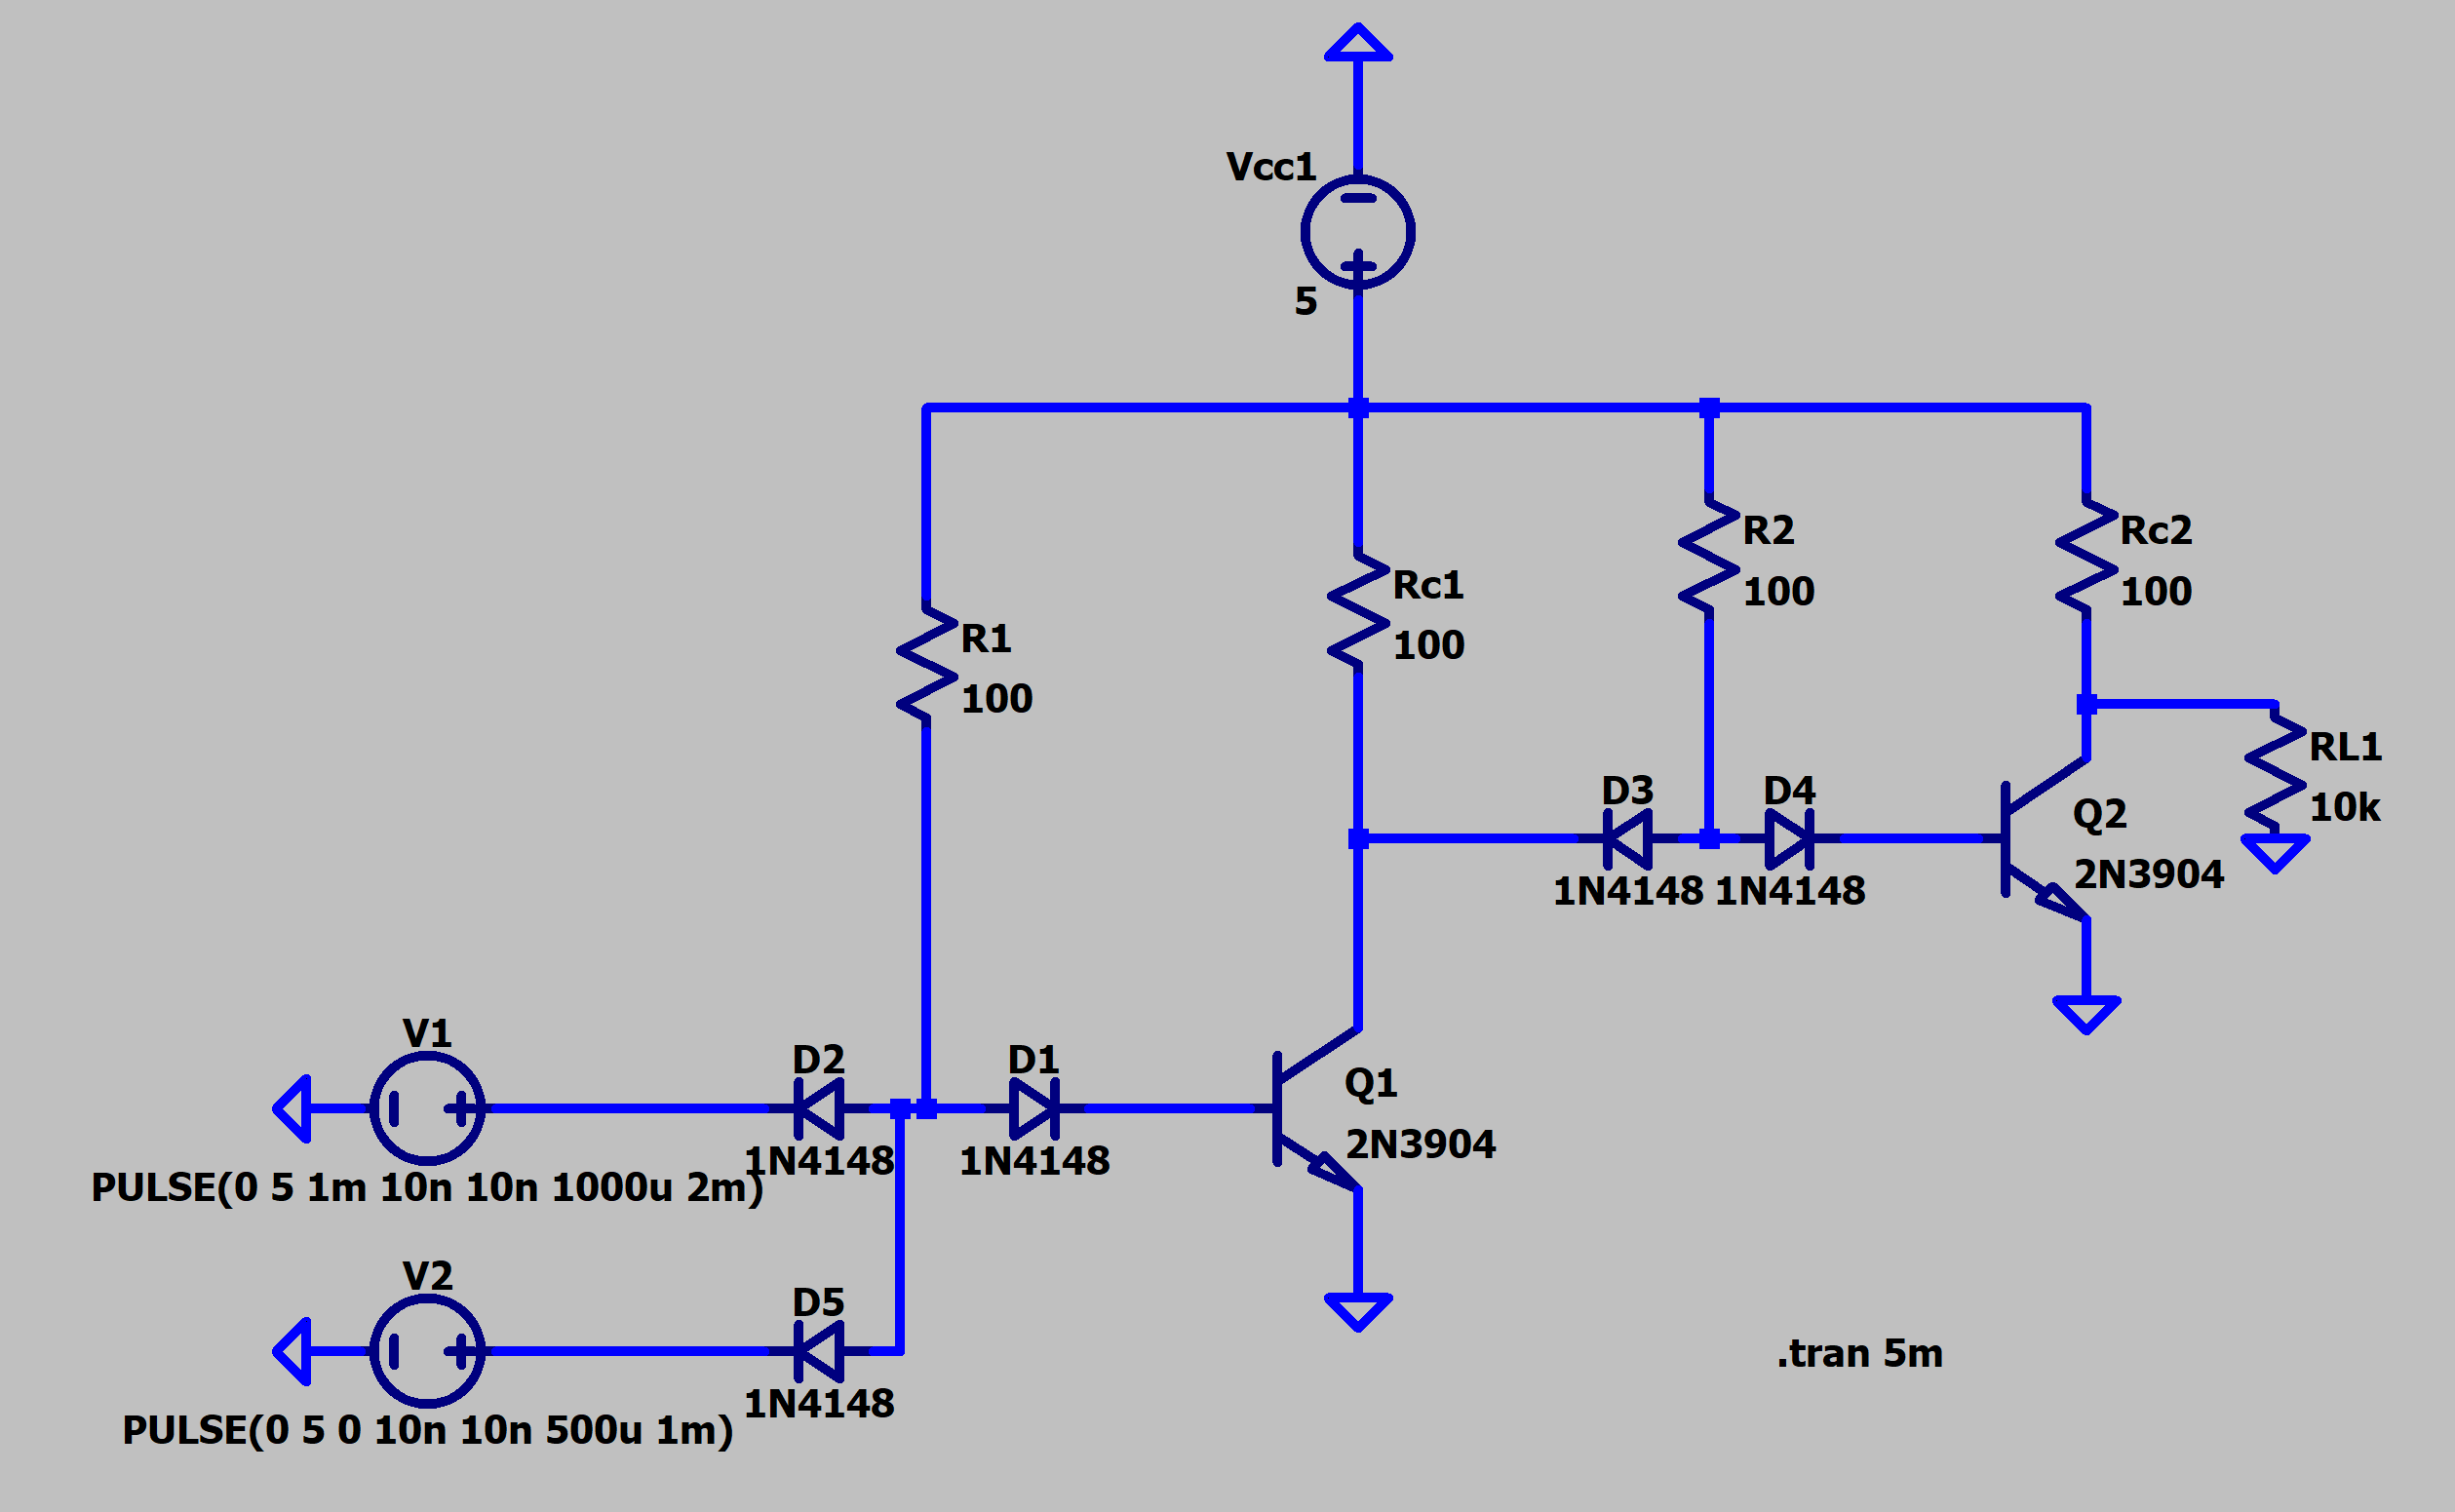
\includegraphics[width=0.7\textwidth]{images/DTL_AND.png}
    \caption{DTL AND}
    \label{DTL_AND}
\end{figure}
\begin{figure}[H]
    \centering
    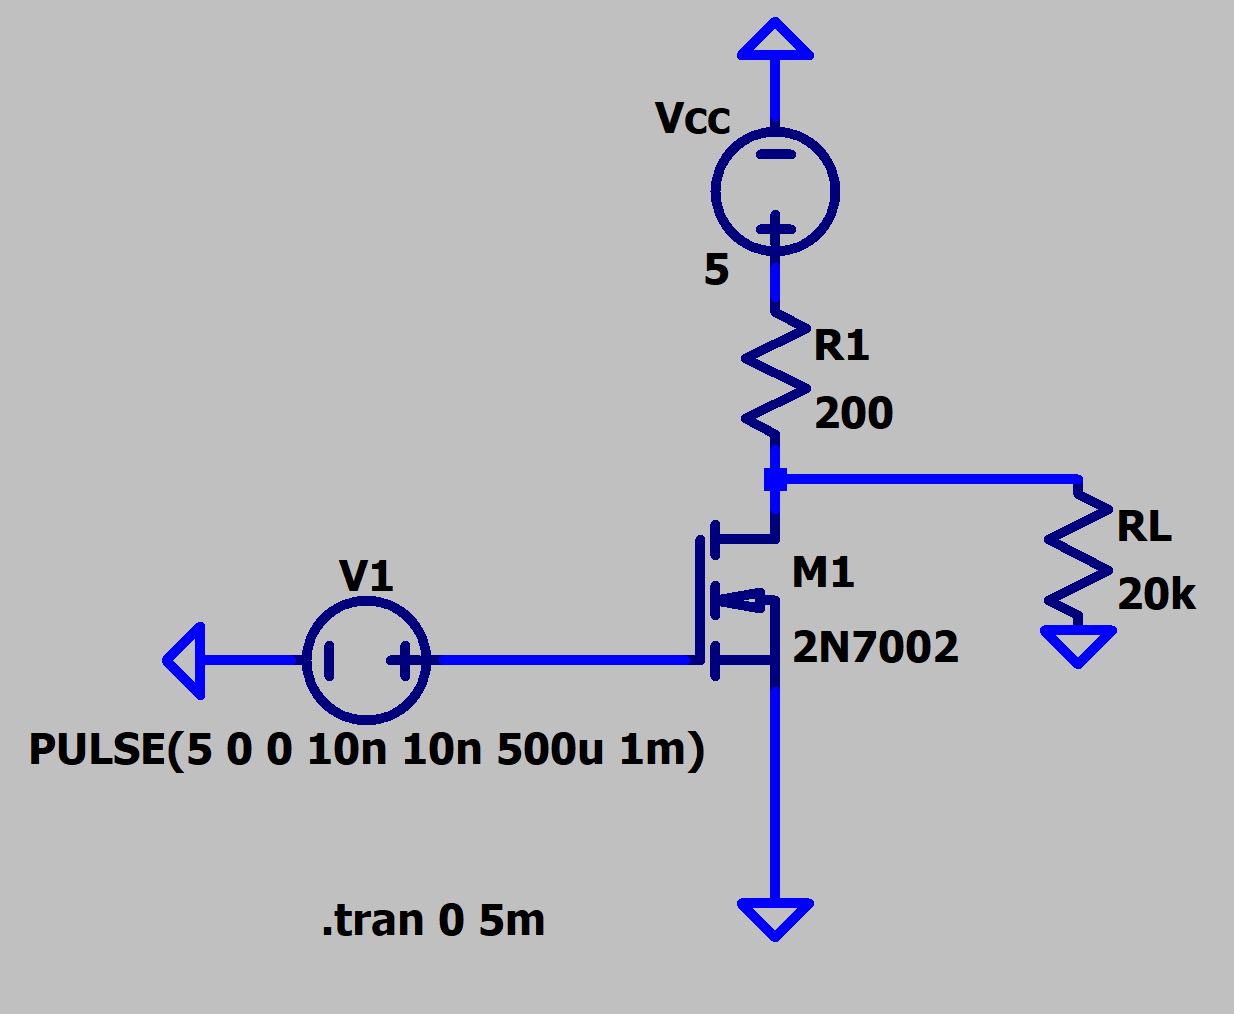
\includegraphics[width=0.5\textwidth]{images/MOS_NOT.png}
    \caption{MOS NOT}
    \label{MOS_NOT}
\end{figure}
\begin{figure}[H]
    \centering
    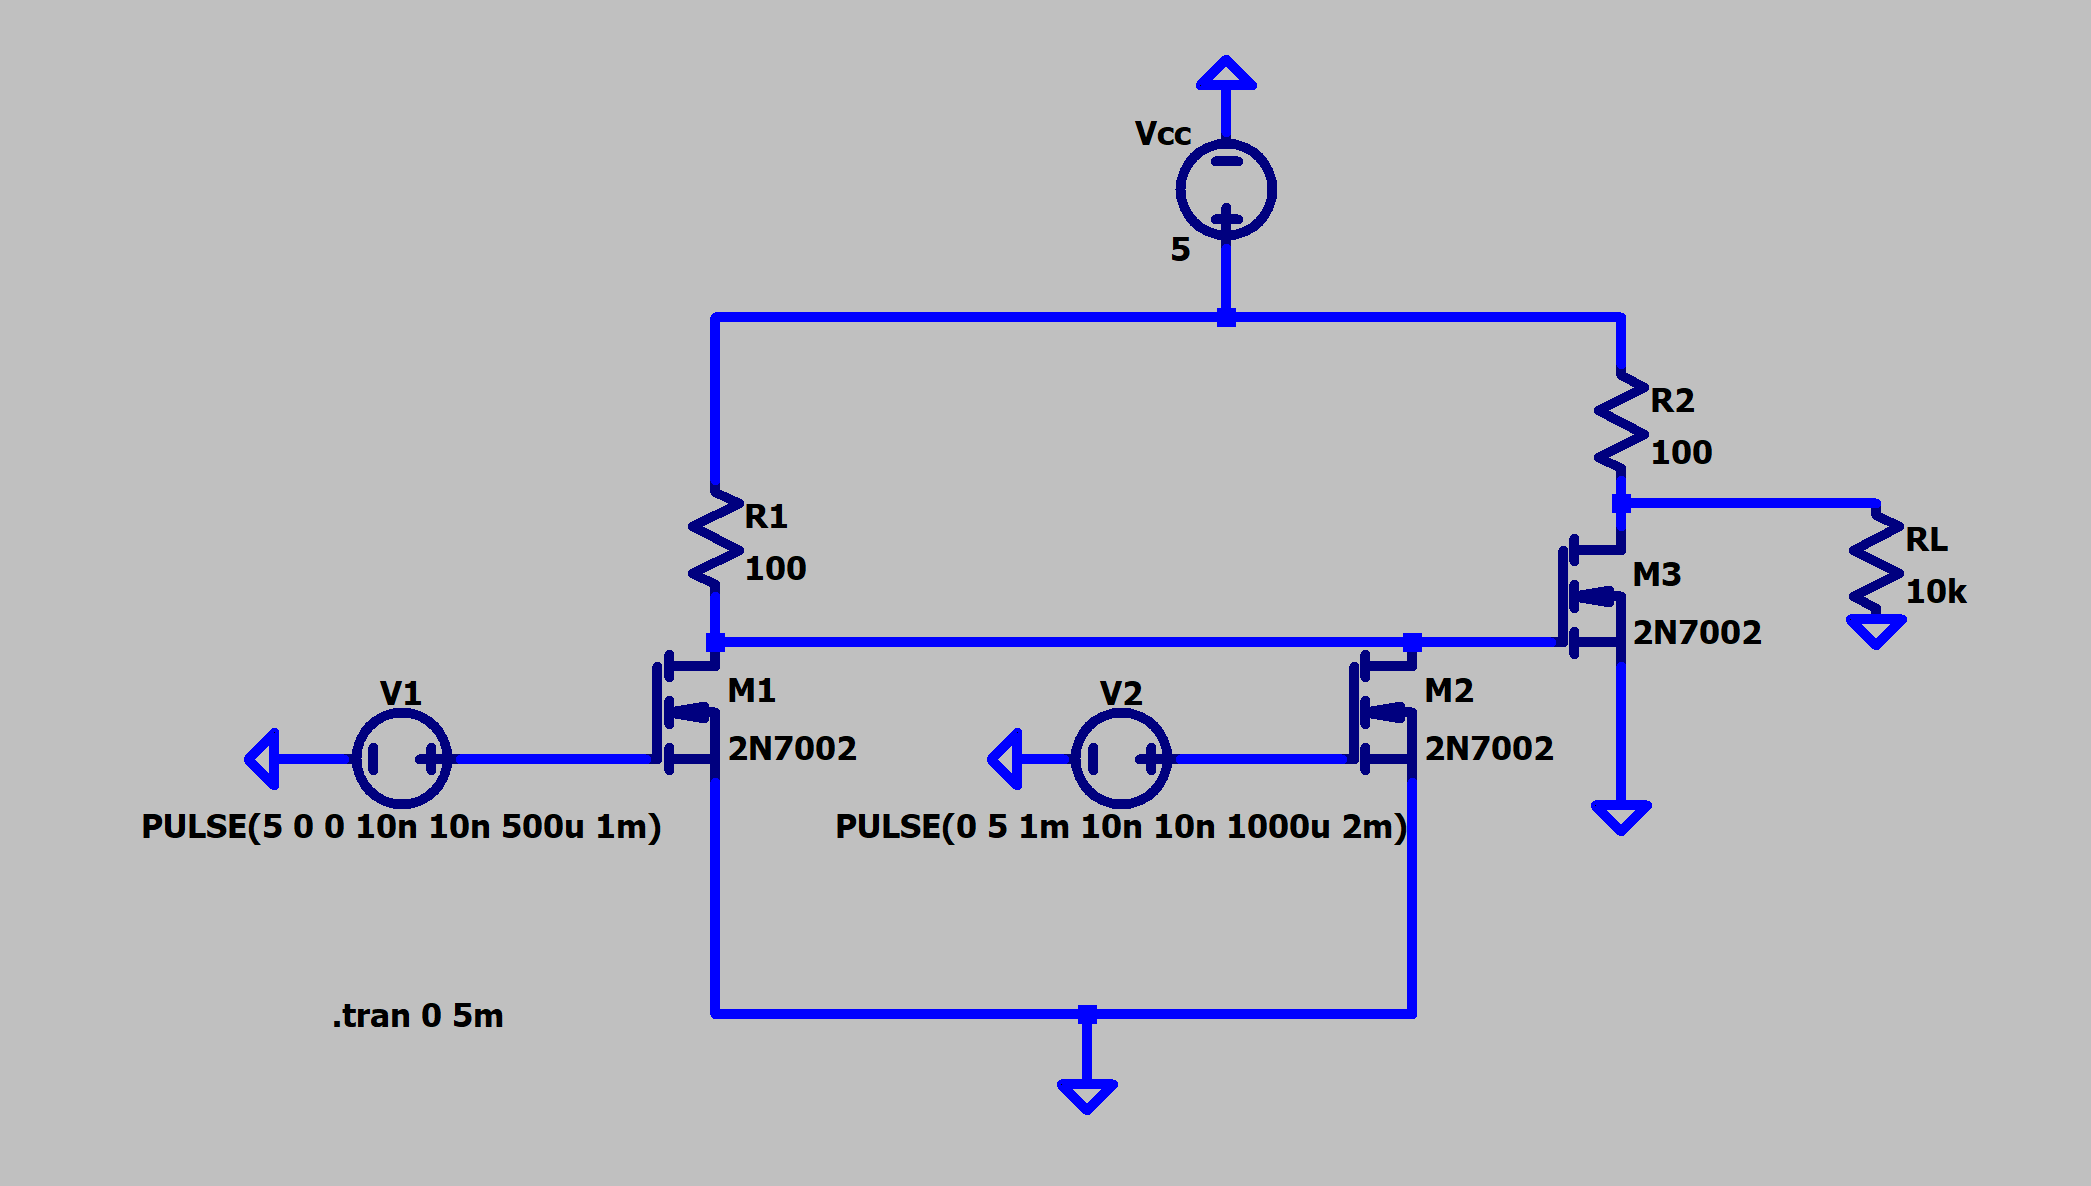
\includegraphics[width=0.9\textwidth]{images/MOS_OR.png}
    \caption{MOS OR}
    \label{MOS_OR}
\end{figure}

\section{Моделирование переходных процессов}
Ниже представлены результаты моделирования переходных процессов:

\begin{figure}[H]
    \centering
    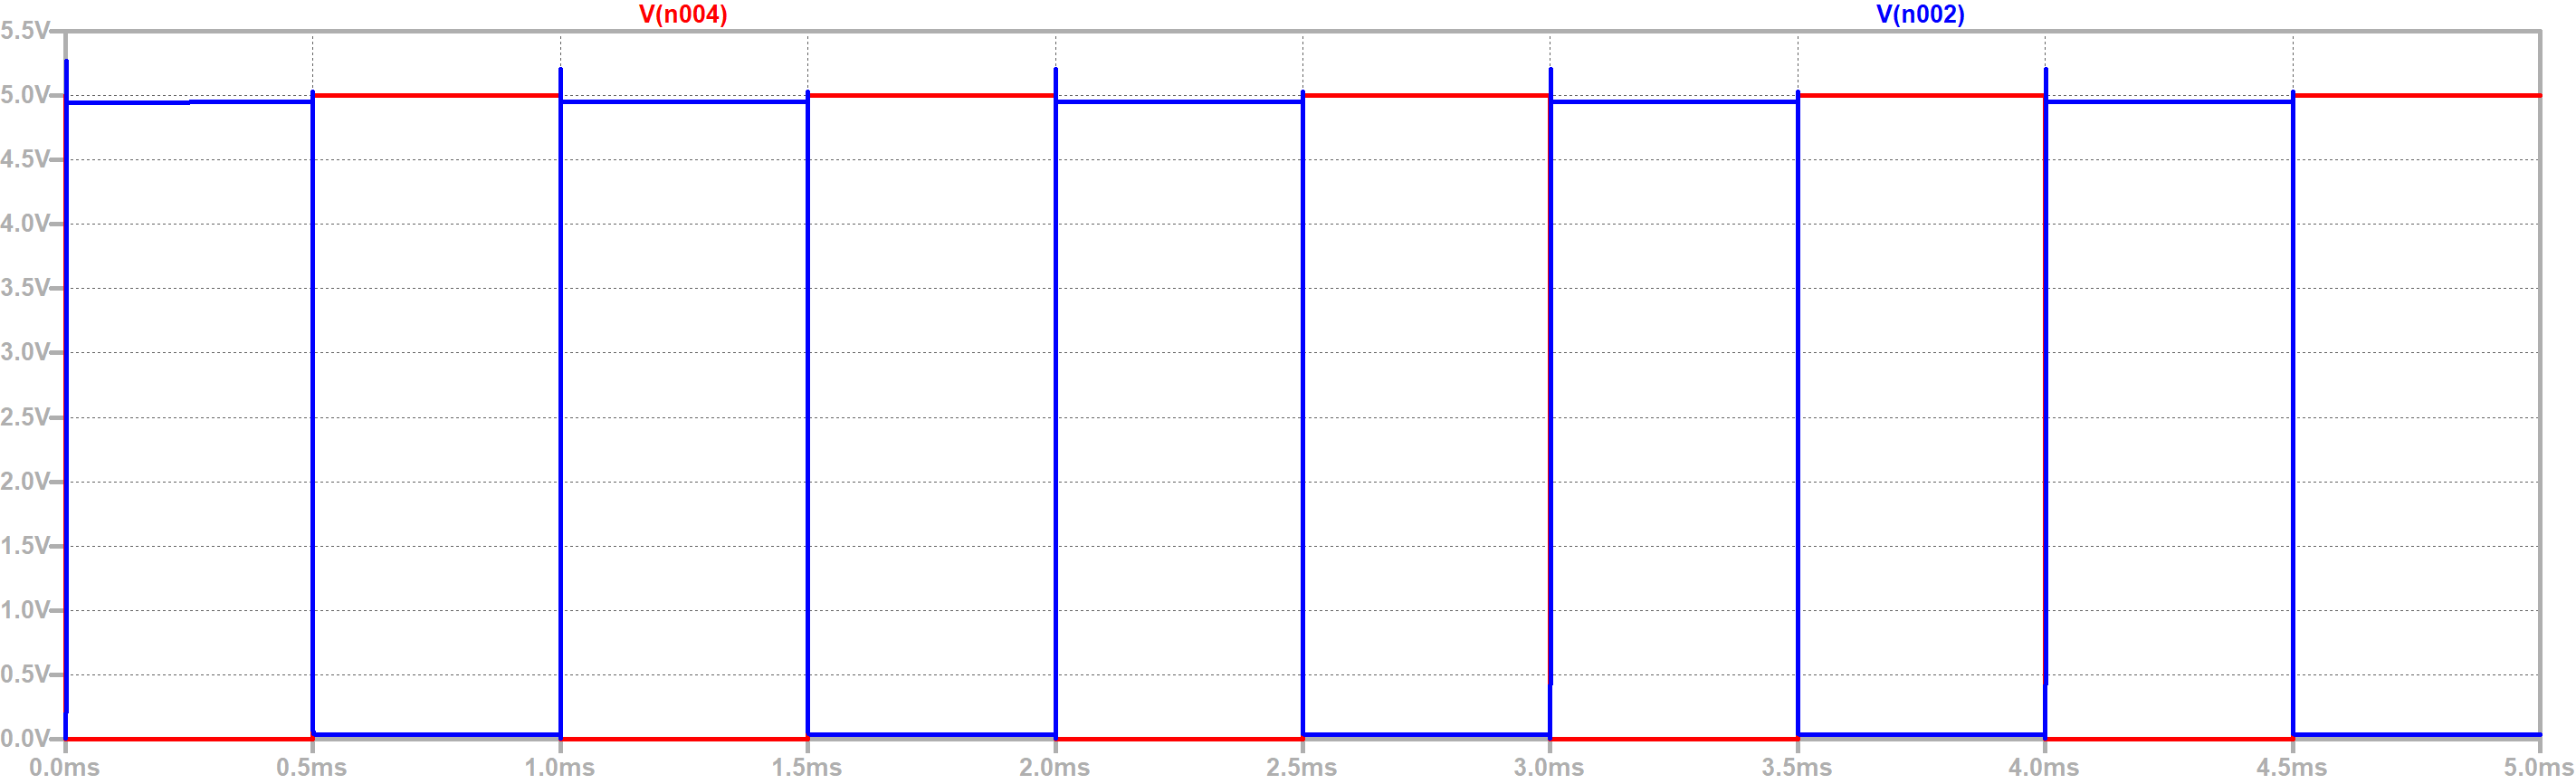
\includegraphics[width=1\textwidth]{images/TTL_NOT_O.png}
    \caption{TTL NOT (Входной сигнал - красный, выходной сигнал - синий)}
    \label{TTL_NOT}
\end{figure}
\begin{figure}[H]
    \centering
    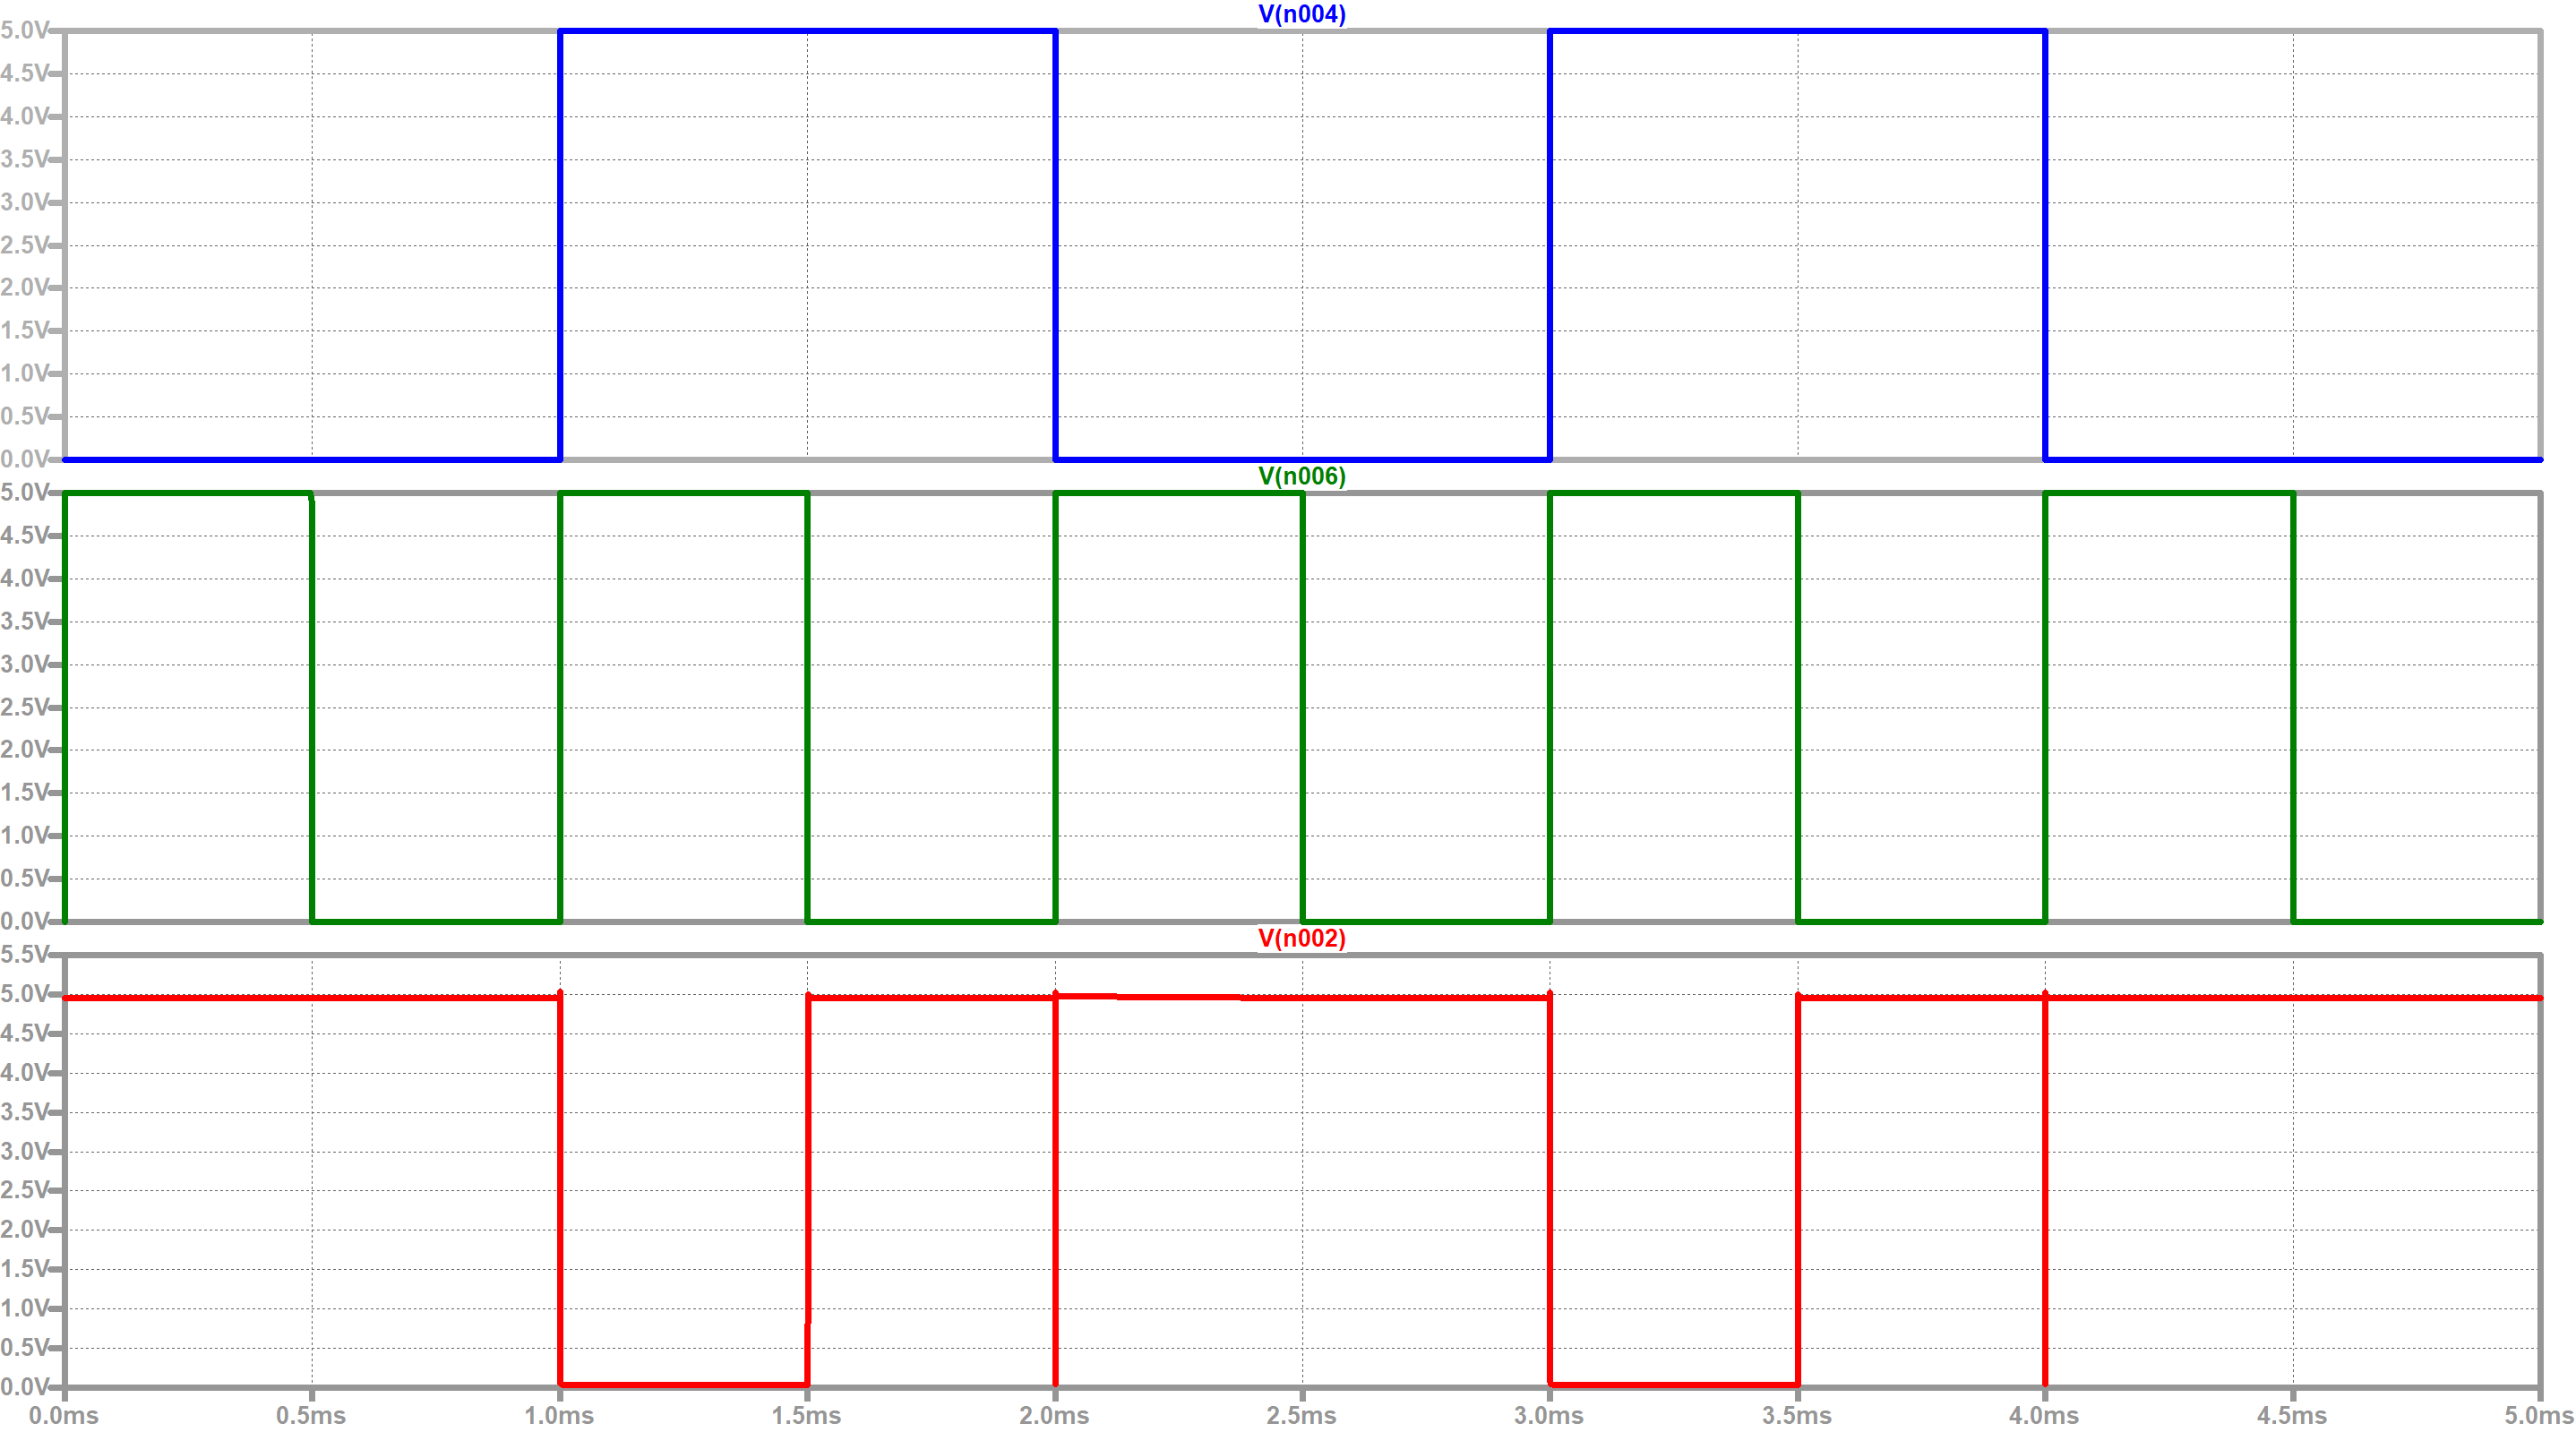
\includegraphics[width=1\textwidth]{images/TTL_NAND_O.png}
    \caption{TTL NAND (V1 - синий, V2 - зеленый, выходной сигнал - красный)}
    \label{TTL_NAND}
\end{figure}
\begin{figure}[H]
    \centering
    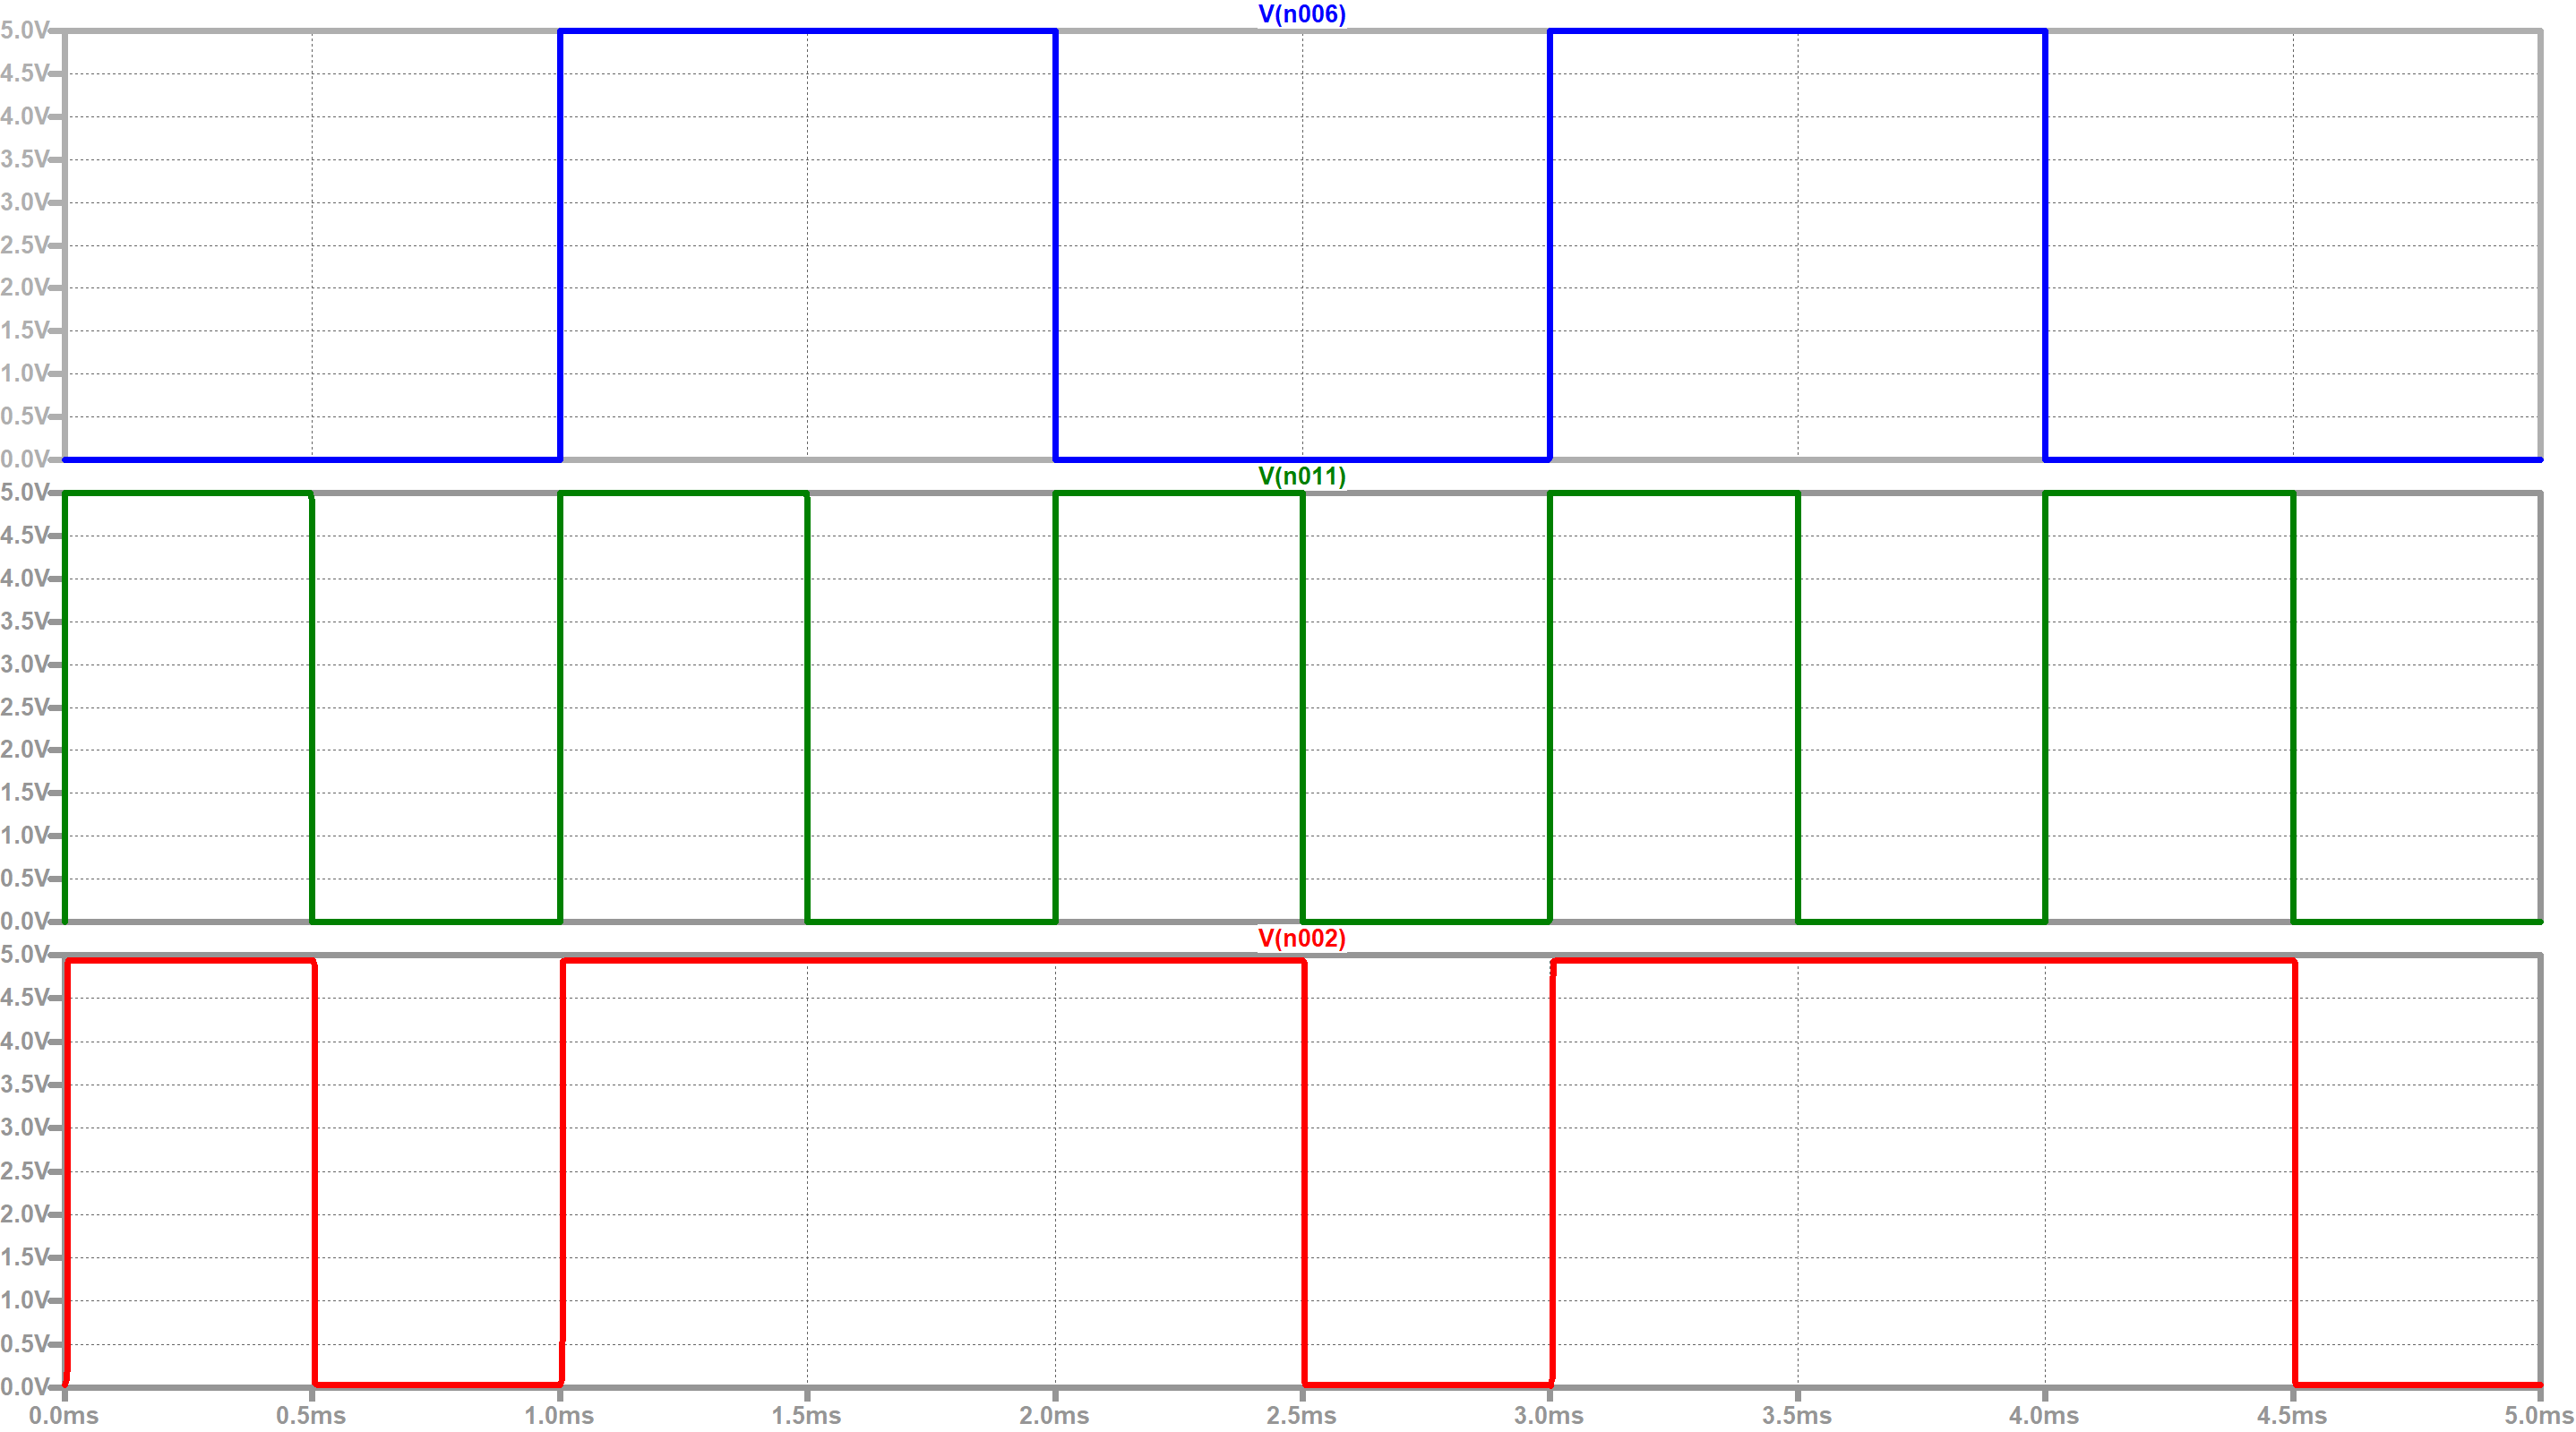
\includegraphics[width=1\textwidth]{images/DTL_OR_O.png}
    \caption{DTL OR (V1 - синий, V2 - зеленый, выходной сигнал - красный)}
    \label{DTL_OR}
\end{figure}
\begin{figure}[H]
    \centering
    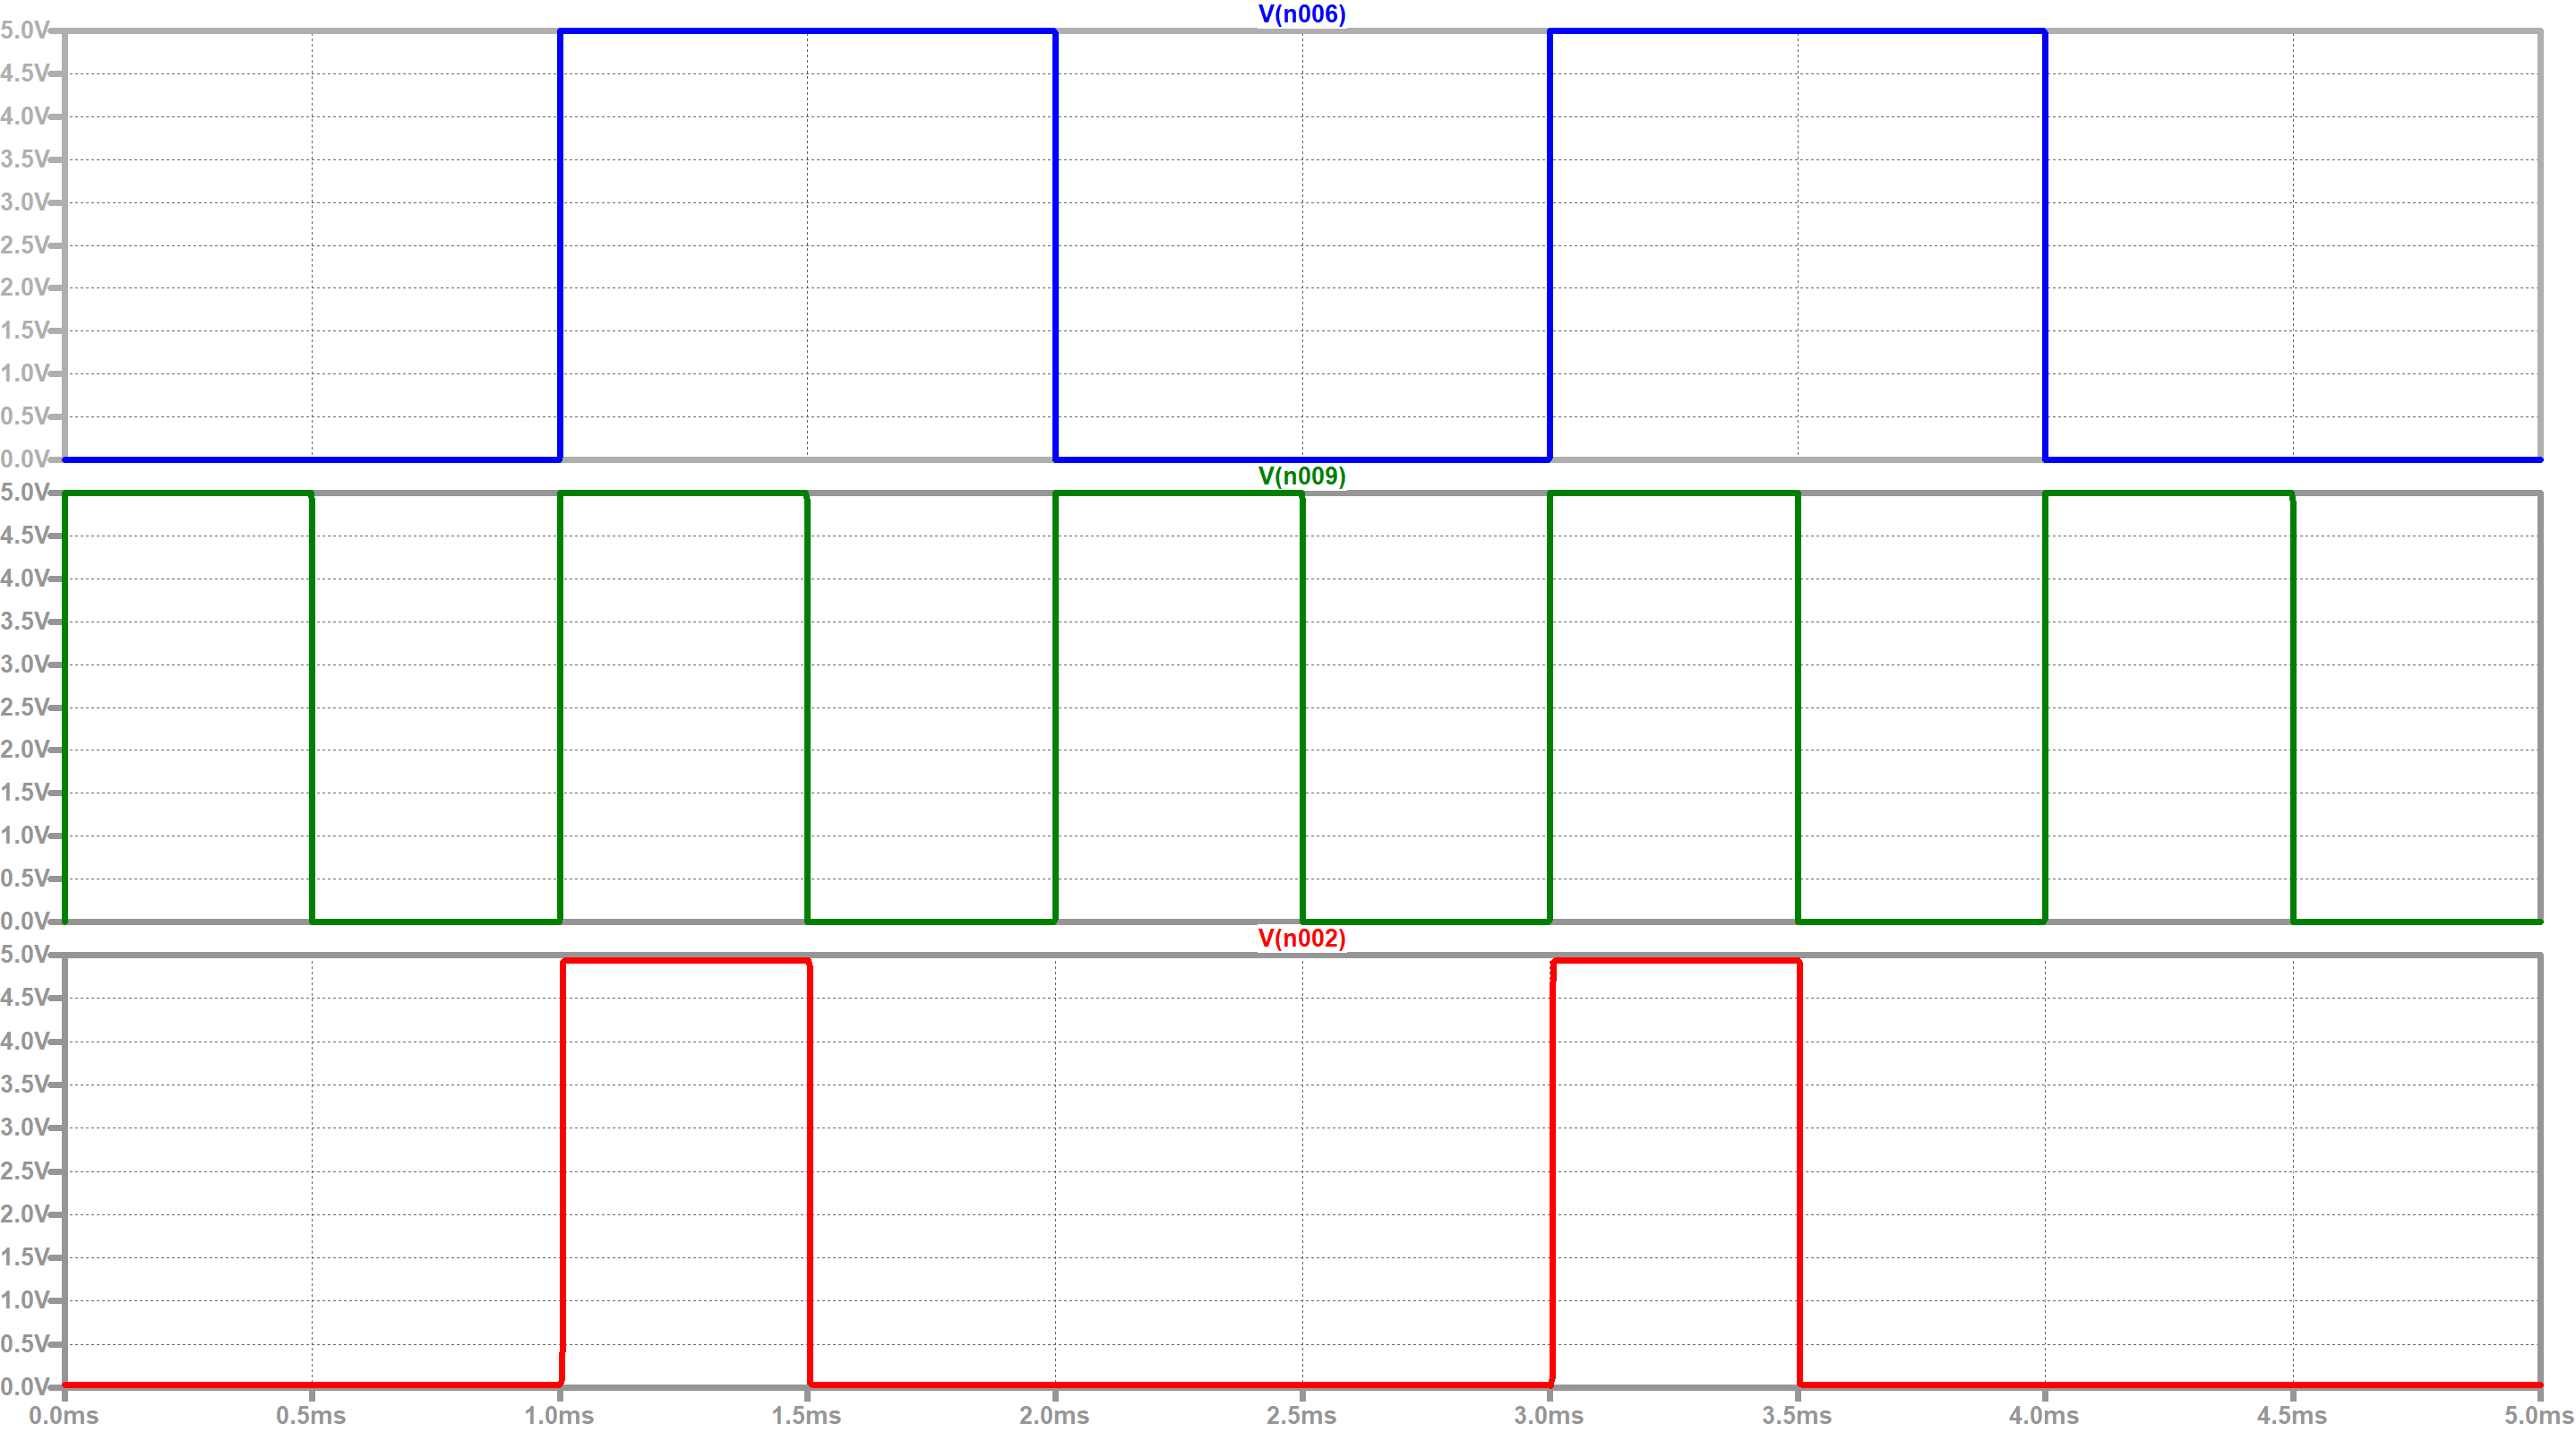
\includegraphics[width=1\textwidth]{images/DTL_AND_O.png}
    \caption{DTL AND (V1 - синий, V2 - зеленый, выходной сигнал - красный)}
    \label{DTL_AND}
\end{figure}
\begin{figure}[H]
    \centering
    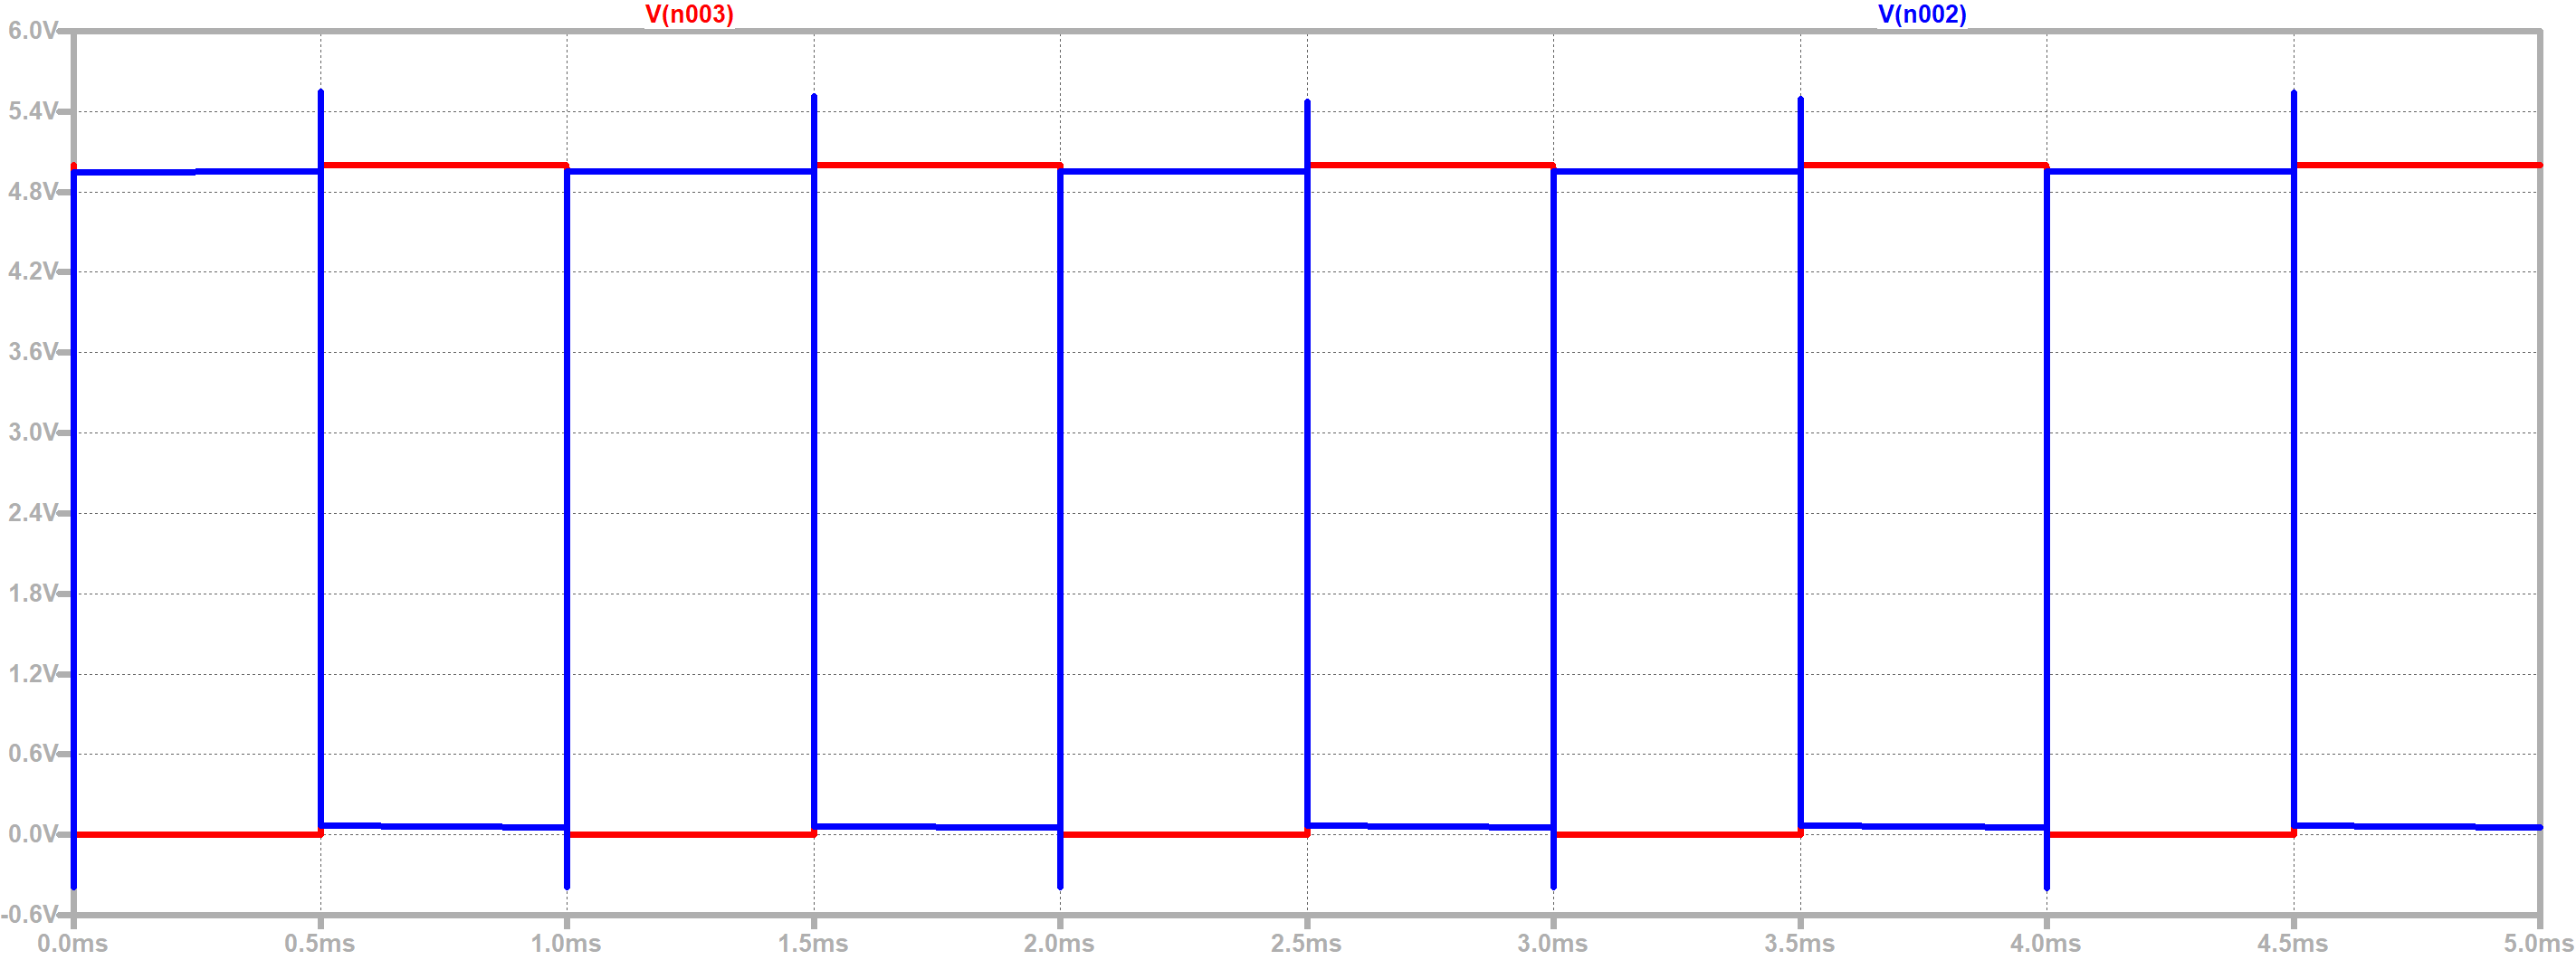
\includegraphics[width=1\textwidth]{images/MOS_NOT_O.png}
    \caption{MOS NOT (Входной сигнал - красный, выходной сигнал - синий)}
    \label{MOS_NOT}
\end{figure}
\begin{figure}[H]
    \centering
    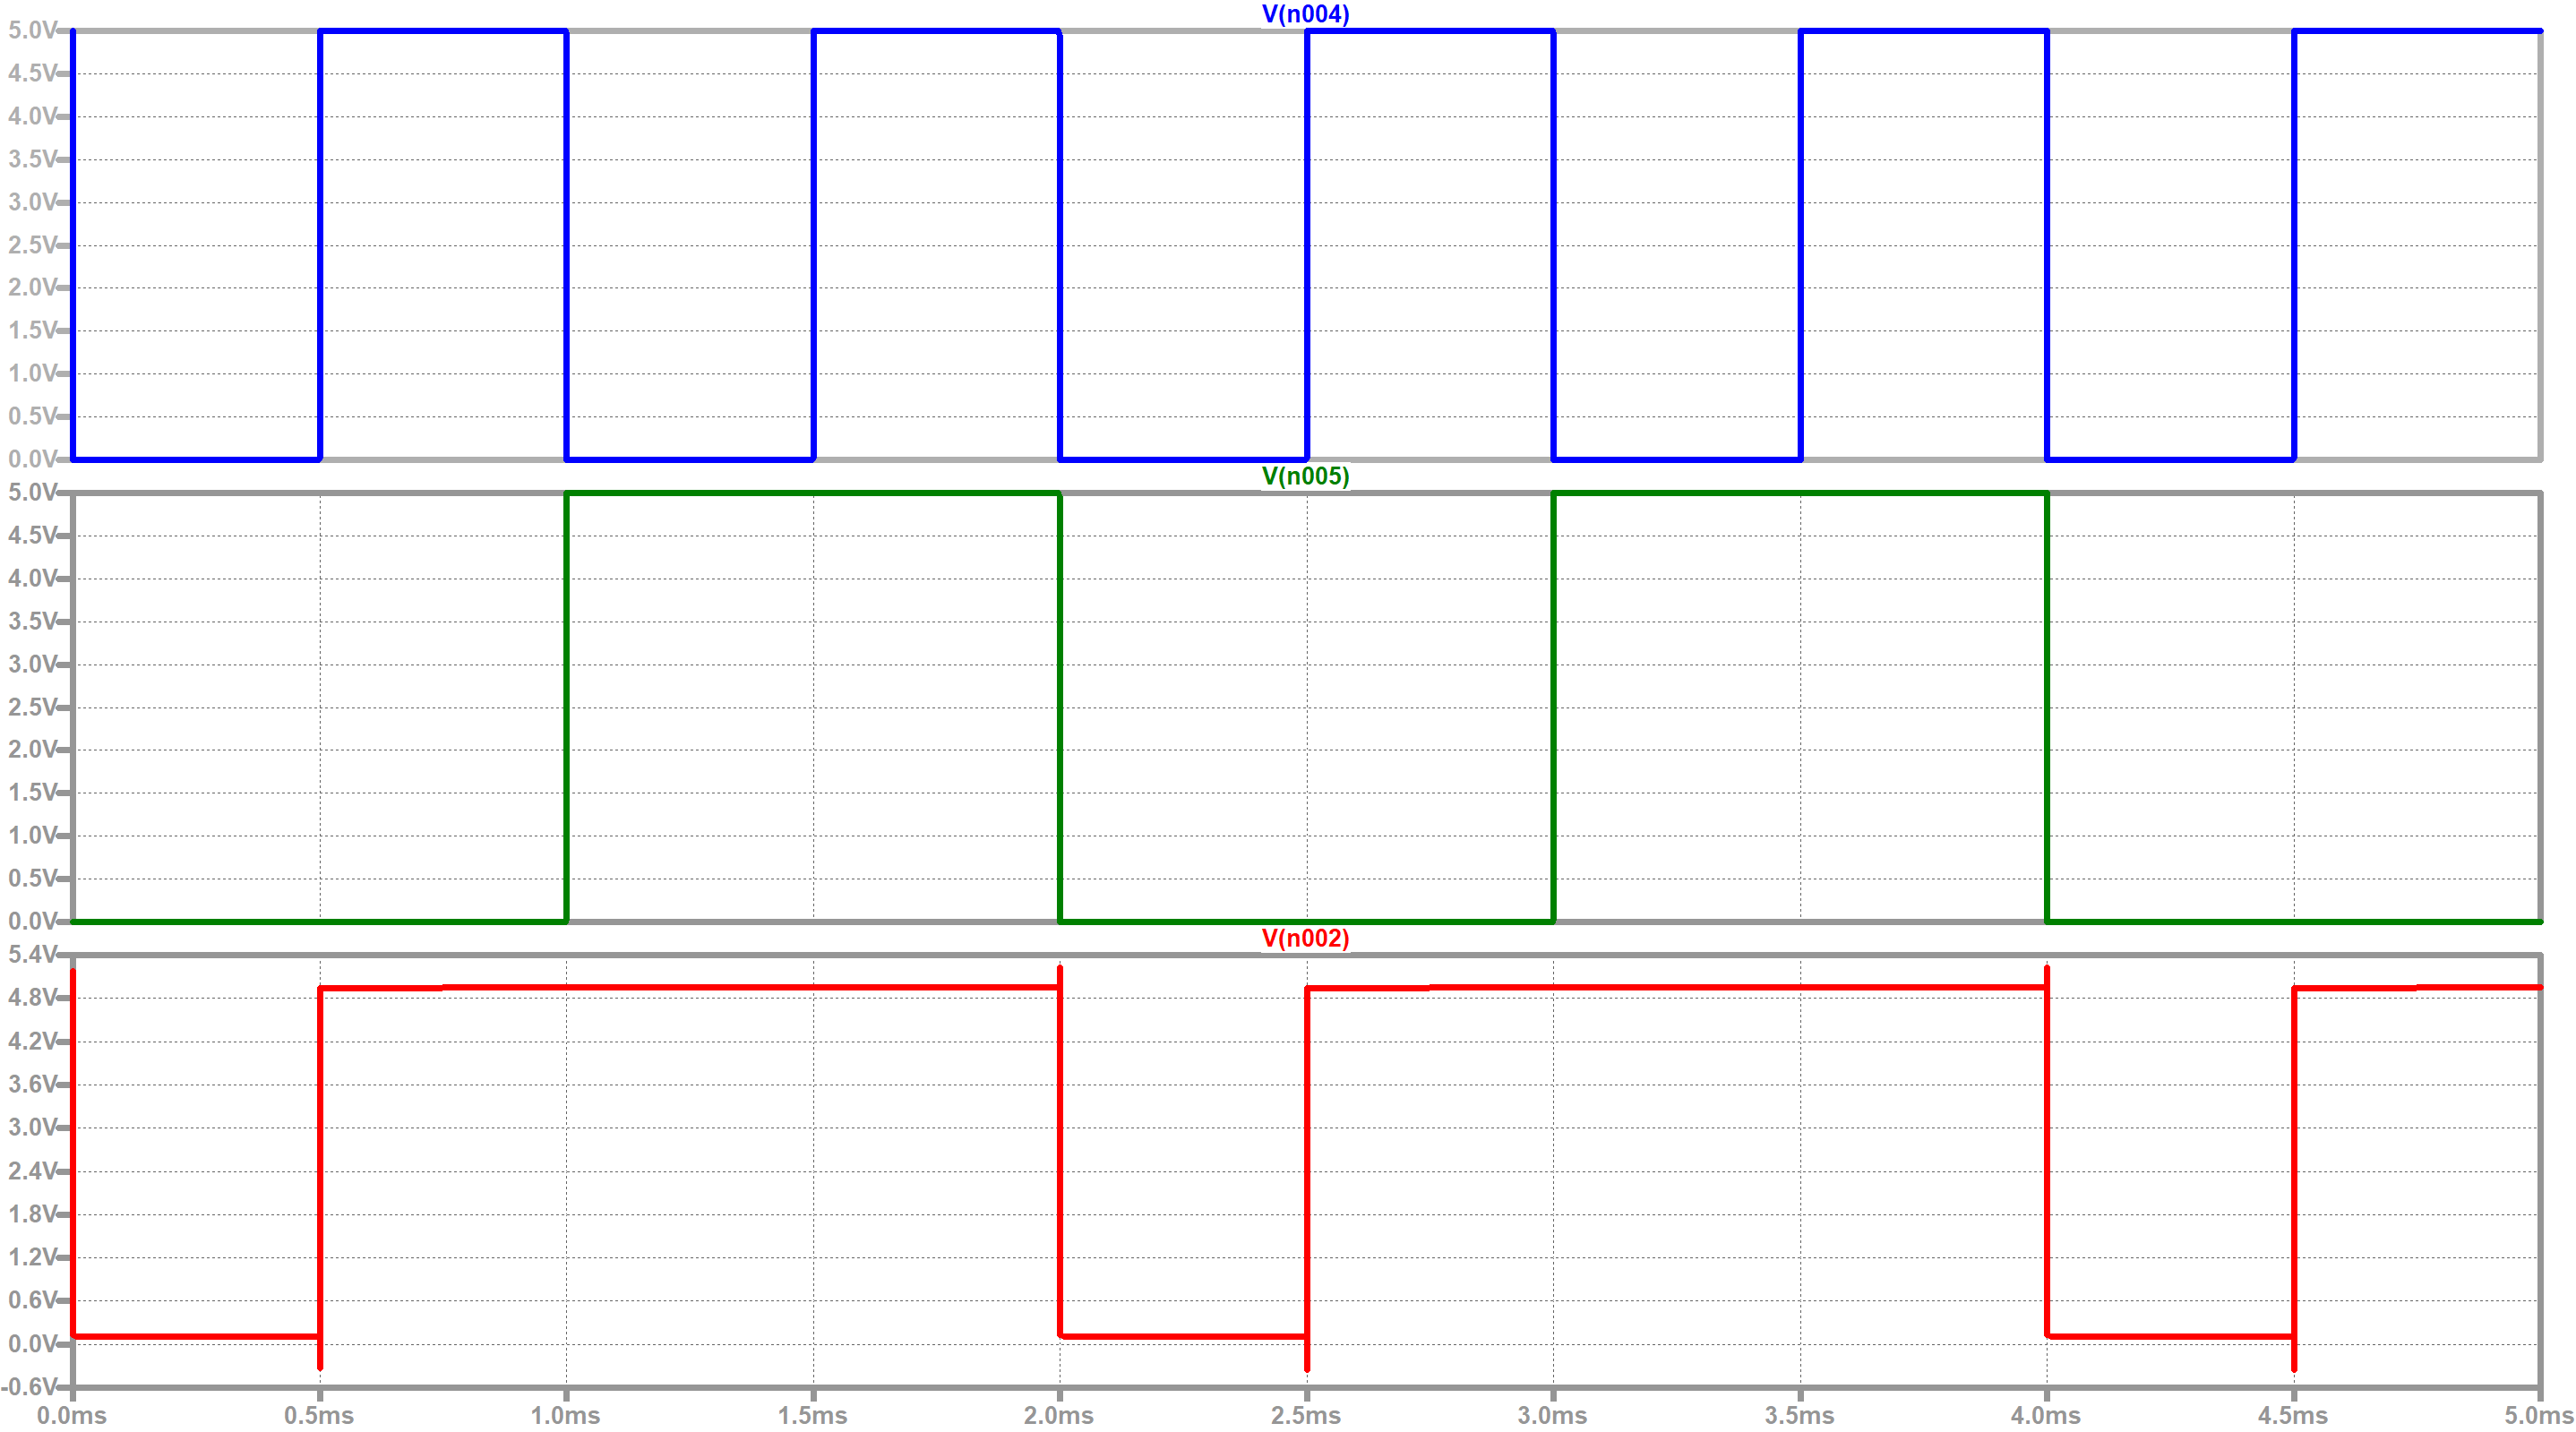
\includegraphics[width=1\textwidth]{images/MOS_OR_O.png}
    \caption{MOS OR (V1 - синий, V2 - зеленый, выходной сигнал - красный)}
    \label{MOS_OR}
\end{figure}

\section{Измерение параметров}
\subsection{TTL NOT}
Уровни:147.53019ns
\begin{itemize}
    \item Логический "0": 0.03V
    \item Логическая "1": 4.95V
\end{itemize}
Времена задержки:
\begin{itemize}
    \item $t_{PLH}$: 1us
    \item $t_{PHL}$: 1us
\end{itemize}
Форма фронтов:
\begin{itemize}
    \item $t_{r}$: Есть короткий выброс при достижении 1
    \item $t_{f}$: Перед началом спада есть небольшой выброс
\end{itemize}
Пиковый ток: 85mA\\
Средний ток: 52.545mA


\subsection{TTL NAND}
Уровни:
\begin{itemize}
    \item Логический "0": 0.03V
    \item Логическая "1": 4.95V
\end{itemize}
Времена задержки:
\begin{itemize}
    \item $t_{PLH}$: 1us
    \item $t_{PHL}$: 3ns
\end{itemize}
Пиковый ток: 89mA\\
Средний ток: 45.498mA


\subsection{DTL OR}
Уровни:
\begin{itemize}
    \item Логический "0": 0.03V
    \item Логическая "1": 4.94V
\end{itemize}
Времена задержки:
\begin{itemize}
    \item $t_{PLH}$: 5us
    \item $t_{PHL}$: 4us
\end{itemize}
Пиковый ток: 216mA\\
Средний ток: 160.5mA


\subsection{DTL AND}
Уровни:
\begin{itemize}
    \item Логический "0": 0.03V
    \item Логическая "1": 4.94V
\end{itemize}
Времена задержки:
\begin{itemize}
    \item $t_{PLH}$: 5us
    \item $t_{PHL}$: 4us
\end{itemize}
Пиковый ток: 187mA\\
Средний ток: 132.89mA


\subsection{MOS NOT}
Уровни:
\begin{itemize}
    \item Логический "0": 0.05V
    \item Логическая "1": 4.95V
\end{itemize}
Времена задержки:
\begin{itemize}
    \item $t_{PLH}$: 15ns
    \item $t_{PHL}$: 2ns
\end{itemize}
Форма фронтов:
\begin{itemize}
    \item $t_{r}$: Перед началом возрастания фронта кратковременое понижение напряжения
    \item $t_{f}$: Перед началом спада есть кратковременый выброс
\end{itemize}
Пиковый ток: 27mA\\
Средний ток: 17.491mA


\subsection{MOS OR}
Уровни:
\begin{itemize}
    \item Логический "0": 0.1V
    \item Логическая "1": 4.95V
\end{itemize}
Времена задержки:
\begin{itemize}
    \item $t_{PLH}$: 12ns
    \item $t_{PHL}$: 30ns
\end{itemize}
Форма фронтов:
\begin{itemize}
    \item $t_{r}$: Перед началом возрастания фронта кратковременое понижение напряжения
    \item $t_{f}$: Перед началом спада есть кратковременый выброс
\end{itemize}
Пиковый ток: 63mA\\
Средний ток: 46.54mA


\section{Сравнительный анализ}

\subsection{Сравнение инверторов TTL и MOS}

\textbf{Общее:} оба элемента корректно выполняют логическую функцию инверсии.

\textbf{Различия:}
\begin{enumerate}
    \item \textbf{Скорость переключения:} MOS-инвертор значительно быстрее (15 нс / 2 нс) против TTL (1 мкс / 1 мкс).
    \item \textbf{Потребление тока:} MOS потребляет в 3 раза меньше тока (27 мА пик, 17.5 мА средн.) чем TTL (85 мА пик, 52.5 мА средн.).
    \item \textbf{Логические уровни:} уровень "0" у MOS выше (0.05 В) чем у TTL (0.03 В).
    \item \textbf{Форма сигнала:} оба имеют выбросы при переключении.
\end{enumerate}

\subsection{Сравнение элементов ИЛИ DTL и MOS}

\textbf{Общее:} оба элемента корректно выполняют логическую функцию ИЛИ.

\textbf{Различия:}
\begin{enumerate}
    \item \textbf{Скорость переключения:} MOS-элемент быстрее (12 нс / 30 нс) чем DTL (5 мкс / 4 мкс).
    \item \textbf{Потребление тока:} MOS потребляет в 3-4 раза меньше тока (63 мА пик, 46.5 мА средн.) чем DTL (216 мА пик, 160.5 мА средн.).
    \item \textbf{Логические уровни:} уровень "0" у MOS выше (0.10 В) чем у DTL (0.03 В).
\end{enumerate}

\subsection{Выводы по логическим семействам}

\begin{enumerate}
    \item \textbf{TTL:} среднее быстродействие, высокое потребление тока, хорошие логические уровни.
    \item \textbf{DTL:} низкое быстродействие, очень высокое потребление тока, хорошие логические уровни.
    \item \textbf{MOS:} высокое быстродействие, умеренное потребление тока, уровень "0" повышен.
\end{enumerate}

MOS-технология показывает преимущества в быстродействии и энергопотреблении, но имеет менее идеальные логические уровни. DTL технология устарела из-за низкого быстродействия и высокого энергопотребления. TTL представляет компромиссный вариант. Однако перечисленные свойства могут меняться в некоторых пределах в зависимости от выбранных компонентов (в частности, резосторов) в схеме.

\section{Общие выводы}

В ходе выполнения работы были исследованы схемы базовых логических элементов (инвертор, И-НЕ, И, ИЛИ), реализованных в трёх логических семействах — TTL, DTL и MOS. Проведено моделирование переходных процессов, измерены ключевые параметры (логические уровни, времена задержки распространения сигнала, форма фронтов, пиковые и средние токи потребления), выполнен сравнительный анализ.

Все исследованные элементы корректно реализуют соответствующие логические функции, что подтверждается осциллограммами переходных процессов.

Логические уровни во всех семействах близки к идеальным (0 В для «0» и 5 В для «1»), однако в MOS-логике уровень логического «0» слегка повышен (0.05-0.1 В), что может снижать помехоустойчивость в некоторых случаях.

Полученные результаты иллюстрируют эволюцию логических семейств: переход от диодно-транзисторных (DTL) и транзисторно-транзисторных (TTL) схем к МОП-структурам позволил существенно повысить быстродействие и снизить энергопотребление при сохранении функциональности.

Таким образом, работа подтверждает целесообразность использования МОП-логики в современных цифровых устройствах и даёт понимание компромиссов, характерных для более ранних семейств. Полученные количественные характеристики могут варьироваться при изменении номиналов компонентов (в первую очередь резисторов), однако общие соотношения между семействами сохраняются.